\documentclass[male, authorStatement, indexNumber, fileVersion, keywords, thanks]{lib/uekthesis}
\usepackage{lib/uekthesis}
\usepackage{pgfplots}
\pgfplotsset{compat=1.17}
\usepackage{tikz}
\usepackage{tikz-cd}
\usetikzlibrary{3d} % Potrzebna do rysowania 3
\usetikzlibrary{positioning}
\usetikzlibrary{shapes.geometric, arrows, positioning, calc}
\tikzstyle{neuron}=[circle,fill=blue!25,minimum size=17pt,inner sep=0pt]
\tikzstyle{input neuron}=[neuron, fill=green!50]
\tikzstyle{output neuron}=[neuron, fill=red!50]
\tikzstyle{hidden neuron}=[neuron, fill=blue!50]
\tikzstyle{annot} = [text width=4em, text centered]

%##############################################################################
% Zmienne Globalne !!! - ważne by kodowanie UTF-8 było wstawione przed nimi
%
% To zmiennne do modyfikacji przez użytkownika
%
\globalFullAuthor{Jan Ślusarek}                      % Pełna nazwa autora pracy
%\globalShortAuthor{J.\ Ślusarek}                     % Autor - zwięzła forma wydruku
\globalFullTitle{Porównanie efektywności metod stochastycznych i algorytmów uczenia maszynowego w optymalizacji portfeli inwestycyjnych \\}  % Pełny tytuł pracy
  % Krótki, zwięzły tytuł pracy
\globalFullUniversity{Uniwersytet Ekonomiczny w Krakowie} % Pełna nazwa uniwersytetu
\globalShortUniversity{UEK}                           % Skrócona nazwa uniwersytetu
\globalDepartment{Instytut Metod Ilościowych w Naukach Społecznych}                % Wydział
\globalDegreeprogramme{Analityka Gospodarcza}         % Kierunek studiów
\globalThesisType{Praca magisterska}                    % Typ pracy dyplomowej
\globalUnderTheSupervisonOf{Pod kierunkiem}
\globalSupervisor{prof. UEK dr hab. Macieja Kostrzewskiego}  % Promotor
%\globalAcknowledgements{Dla moich rodziców oraz najbliższych przyjaciół za niezłomną wiarę w~moje zwycięstwo.}   % Podziękowania
\globalIndexNumber{215302}  % wersja pliku
%\globalCity{Kraków}         % miasto
%\globalYear{2024}           % rok powstania pracy
%\globalKeywords{nauka, komputery, praca dyplomowa, latex, uczelnia, student} % słowa kluczowe dla pracy

%##############################################################################
% Dołączenie pliku bibliografii zgodnej z Biblatex
\addbibresource{bibliography.bib}

%##############################################################################
% dodatkowe pakiety
\usepackage{chemfig} % wzory chemiczne

% Lista słów (dzielenia je, lub nie)
\hyphenation{LaTeX latex LaTeXu}

%##############################################################################
% Koniec preambuły i rozpoczęcie treści właściwej dokumentu
\begin{document}
\nocite{*}

\titlepages
\tableofcontents
%\clearpage

% Tu umieszczamy rozdziały w porządanej kolejności 
\chapter*{Wstęp}
\label{chap:wstep}
\addcontentsline{toc}{chapter}{Wstęp}
\addtocounter{chapter}{0}
\sectionmark{Wstęp} % changes the head for the current page





\chapter{Matematyczne podwaliny budowy portfela}
\label{chap:teoretyczne_podwaliny}
\section{Modelowanie ciągłych procesów stochastycznych w finansach}
Koncepcja modelowania danych czasowych jest jedną z klasycznych aplikacji matematyki w naukach empirycznych. Za bardzo umowny początek tych metod, uznać możemy (nie umniejszając Leibnitzowi)\textit{Philosophiae naturalis principia mathematica} autorstwa angielskiego fizyka Isaaca Newtona\footnote{M. Waszczyk, E. Szczerbicki, \textit{Metodologiczne Aspekty Opisowego Modelowania w Naukach Ekonomicznych}, Zeszyty Naukowe Politechniki Gdańskiej, nr. 30, s.17}. Newton w swych pracach ustanowił podstawy mechaniki klasycznej, wprowadzając prawa ruchu oraz prawo powszechnej grawitacji. Te fundamentalne prawa miały ogromny wpływ nie tylko na rozwój nauki, ale i na praktyczne zastosowania w inżynierii. Skuteczność teorii Newtona dały podstawy filozofii determinizmu, która głosiła że możliwe jest precyzyjne określenie kauzalności każdego znanego nam stanu i procesu. Determinizm jako paradygmat odcisnął olbrzymi ślad w filozofii oświeceniowej, a jego implikacje były szczególnie widoczne w nukach humanistycznych, które błędnie zaczęły implementować metody mechanistyczne do złożonych procesów rzeczywistości\footnote{A. Staruszkiewicz, \textit{Izaak Newton a Oświecenia Francuskie}, Foton, nr. 107, s. 33-46}. Załamanie się tej koncepcji przychodzi na przełomie XIX i XX wieku za sprawą francuskiego naukowca Henri'ego Poincaré wraz z jego słynnym problemem n ciał\footnote{M. Heller, \textit{Rewolucja probabilistyczna}, Studies in History and Philosophy of Modern Physics, nr. 38, s. 204-218}. Problem ten brzmi następująco: Jak będzie się poruszać \(n\) ciał, które oddziałują na siebie wzajemnie siłami grawitacji? W przypadku kiedy jest jedno ciało to po prostu znajduje się w spoczynku. Kiedy dane są dwa ciała rozwiązaniem jest trajektoria eliptyczna lub paraboliczna, jest to wtedy tzw. Prawo Keplera. Jednakże kiedy liczba ciał wynosi 3, nie istnieje rozwiązanie tego problemu w formie analitycznej. Wynika to z tego że małe zmiany w warunkach początkowych mogą prowadzić do dramatycznie różnych trajektorii ruchu. Obserwacja ta dała początek w formułowaniu procesów stochastycznych które jako jeden z pierwszych sformułował uczeń Poincaré'go Louis Bachelier, który użył ich w teorii spekulacji\footnote{L. Bachakier, \textit{Théorie de la spéculation}, Annales scientifiques de l’É.N.S, seria 17, tom 3, s. 21-86}. 
Procesy o naturze stochastycznej możemy rozumieć jako ewolucje systemu w czasie rządzoną przez prawa prawdopodobieństwa, a więc struktura tych procesów jest odmienna od procesów deterministycznych. Kardynalna różnica filozoficzna polega na tym że o ile proces deterministyczny jesteśmy w stanie prognozować bez błędu, gdyż znamy wszystkie warunki początkowe. O tyle w przypadku procesów stochastycznych tych warunków nie znamy, a więc prognozujemy zawsze z ryzykiem błędu.
Niech \((\Omega, \mathcal{F}, P)\) będzie przestrzenią probabilistyczną, a \( T \) zbiorem indeksów reprezentującym czas. Proces stochastyczny \((X_t)_{t \in T}\) jest zdefiniowany jako\footnote{M. Pitera, \textit{Procesy Stochastyczne -notatki z wykładu- (2022/2023)}, Kraków 2023, s. 7}:
\begin{equation}
\forall t \in T, \quad X_t: \Omega \to \mathbb{R}^n,
\end{equation}
gdzie:
\begin{itemize}
  \item \(\Omega\) jest przestrzenią zdarzeń,
  \item \(\mathcal{F}\) jest \(\sigma\)-ciałem na \(\Omega\),
  \item \(P\) jest miarą prawdopodobieństwa na \((\Omega, \mathcal{F})\),
  \item \(T\) jest zbiorem indeksów, zwykle reprezentującym czas (np. \( T \) może być przedziałem czasowym lub zbiorem dyskretnym momentów czasowych),
  \item \(t\) jest elementem zbioru \(T\) i reprezentuje konkretny moment w czasie,
  \item \(X_t(\omega)\) jest wartością procesu w momencie \(t\) dla zdarzenia \(\omega \in \Omega\),
  \item \(n\) jest wymiarem przestrzeni stanów procesu.
\end{itemize}

Obrazując to na przykładzie tematycznym, rozważmy cenę akcji pewnej firmy, która zmienia się każdego dnia handlowego. 
Niech \((\Omega, \mathcal{F}, P)\) będzie przestrzenią probabilistyczną, gdzie:
\begin{itemize}
  \item \(\Omega\) reprezentuje wszystkie możliwe ścieżki zmian cen akcji w czasie,
  \item \(\mathcal{F}\) jest \(\sigma\)-ciałem zawierającym zdarzenia związane ze zmianami cen,
  \item \(P\) jest miarą prawdopodobieństwa, która przypisuje szanse różnym zdarzeniom rynkowym.
\end{itemize}

Niech \(T\) oznacza zbiór indeksów reprezentujących dni handlowe na giełdzie, a \(X_t\) cenę akcji w dniu \(t\). Wtedy proces stochastyczny \((X_t)_{t \in T}\) jest zdefiniowany jako:
\newtheorem{theorem}{Twierdzenie}
\newtheorem{lemma}[theorem]{Lemat}
\newtheorem{definition}[theorem]{Definicja}
\begin{theorem}
%\forall t \in T, \quad X_t: \Omega \to \mathbb{R}
\end{theorem}

\begin{equation}
\forall t \in T, \quad X_t: \Omega \to \mathbb{R},
\end{equation}
gdzie \(X_t(\omega)\) to cena akcji w dniu \(t\) dla danej trajektorii \(\omega \in \Omega\). 
W tym modelu, cena akcji \(X_t\) każdego dnia jest wartością numeryczną, która wahania się losowo w zależności od różnych czynników rynkowych. Chociaż ogólne trendy rynkowe mogą być znane, codzienne fluktuacje cen są nieprzewidywalne i podlegają losowości.

Procesy stochastyczne możemy zaklasyfikować ze względu na zbiór indeksów \(T\). Istnieją bowiem dwa przypadki kiedy zakładamy że: \( t \in \mathbb{R} \) albo \( t \in \mathbb{N} \). Prymat historyczny mają tutaj procesy czasu ciągłe, a konkretnie proces Wienera-Bacheliera\footnote{J. Zabczyk, \textit{Ważniejsze wydarzenia w teorii procesów stochastycznych}, Roczniki Polskiego Towarzystwa Matematycznego, Seria II: Wiadomości Matematyczne XL (2004), s. 78}. Pojawił się niezależnie od siebie w pracach badaczy z zakresu finansów oraz fizyki teoretycznej. Wspomniany przeze mnie na poprzedniej stronie, uczeń Poincaré'go w 1900 roku opublikował go w pracy poświęconej analizie cen na giełdzie paryskiej. Niestety jego praca niesłusznie nie została w tych czasach doceniona. Świadczy o tym fakt że za odkrywce tego procesu uznawany jest Nobert Wiener, który sformalizował ten zapis ponad 20 lat później. Groteski dodaje fakt że, podzielił w pewnym sensie los swojego mistrza, który pomimo bycia prekursorem teorii względności nie został dostatecznie doceniony przez ówczesne środowisko intelektualne. Niezależnie od tych badaczy proces ten sformułował również Marian Smoluchowski oraz Albert Einstein w pracach nad modelowaniem ruchów Browna. Proces Wienera-Bachaliera \( W(t) \), dla \( t \geq 0 \), jest zdefiniowany jako\footnote{J. Jakubowski, R. Sztencel, \textit{Wstęp do teorii prawdopodobieństwa}, Warszawa 2003, s. 304-311}:
\begin{equation}
    W(0) = 0, \quad \text{a dla } t > 0, \quad W(t) \text{ jest ciągły i posiada niezależne przyrosty.}
\end{equation}
Dla \( s < t \), przyrosty procesu Wienera-Bachaliera są normalnie rozłożone z wartością oczekiwaną 0 i wariancją proporcjonalną do długości przedziału czasu:
\begin{equation}
    W(t) - W(s) \sim \mathcal{N}(0, t - s).
\end{equation}

\begin{itemize}
  \item \( W(t) \) oznacza wartość procesu Wienera-Bachaliera w chwili \( t \).
  \item \( W(s) \), gdzie \( s \) jest dowolnym momentem czasowym mniejszym niż \( t \), reprezentuje wartość procesu Wienera w chwili \( s \).
  \item \( t \) i \( s \) są zmiennymi reprezentującymi czas, z zakresu \( t \geq 0 \) i \( s < t \).
  \item \( \mathcal{N}(0, t - s) \) oznacza rozkład normalny z wartością oczekiwaną 0 i wariancją \( t - s \).
\end{itemize}
Proces Wienera-Bachaliera charakteryzuje się ciągłością trajektorii oraz niezależnością i stacjonarnością przyrostów. Alternatywnie proces ten można zapisać jeszcze w postaci stochastycznego równania różniczkowego\footnote{}. Rozważmy przyrost \( \Delta Z(t) = Z(t) - Z(t - \Delta t) \) w krótkim przedziale czasu \( \Delta t \). Z uwagi na właściwości procesu Wienera, \( \Delta Z(t) \) jest zmienną losową o rozkładzie normalnym \( N(0, \Delta t) \). Możemy przedstawić \( \Delta Z(t) \) za pomocą zmiennej losowej \( \epsilon \) o standardowym rozkładzie normalnym \( N(0, 1) \), skalując ją przez \( \sqrt{\Delta t} \), co prowadzi do wyrażenia \( \Delta Z(t) = \epsilon \sqrt{\Delta t} \).

W kontekście stochastycznego równania różniczkowego, gdy \( \Delta t \) dąży do zera, stosujemy notację różniczkową:
\begin{equation}
dW_t = \epsilon_t \sqrt{dt}
\end{equation}
gdzie \( \epsilon_t \) jest standardowym białym szumem (szumem gaussowskim z niezależnymi, identycznie rozłożonymi przyrostami), a \( dt \) reprezentuje nieskończenie mały przyrost czasu.
\begin{figure}
\centering
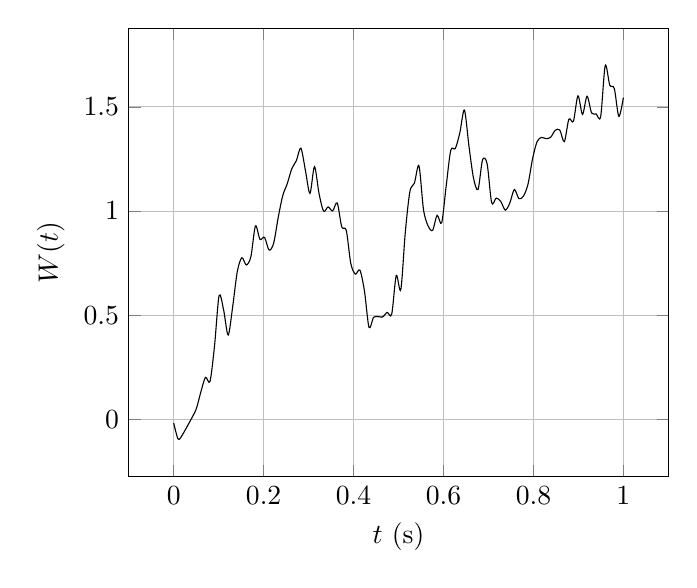
\begin{tikzpicture}
\begin{axis}[
    xlabel={$t$ (s)},
    ylabel={$W(t)$},
    grid=major]
    \addplot[smooth] coordinates {
         (0.0, -0.016086799764720865) (0.010101010101010102, -0.09410211955415858) (0.020202020202020204, -0.07011589313134992) (0.030303030303030304, -0.03166905904307489) (0.04040404040404041, 0.00820352821914936) (0.05050505050505051, 0.05300615664396759) (0.06060606060606061, 0.13394696257227276) (0.07070707070707072, 0.20225405476867117) (0.08080808080808081, 0.18372543903361613) (0.09090909090909091, 0.35535886283506046) (0.10101010101010102, 0.5946266346786072) (0.11111111111111112, 0.524967822136937) (0.12121212121212122, 0.4057278449900589) (0.13131313131313133, 0.5432857088725529) (0.14141414141414144, 0.7092544281722728) (0.15151515151515152, 0.7762999261225444) (0.16161616161616163, 0.7415942437031295) (0.17171717171717174, 0.7815950945792126) (0.18181818181818182, 0.9284051145510913) (0.19191919191919193, 0.8639431252469453) (0.20202020202020204, 0.8738615364440191) (0.21212121212121213, 0.8130073064549687) (0.22222222222222224, 0.8452038052815953) (0.23232323232323235, 0.9676781438646704) (0.24242424242424243, 1.0734356674521233) (0.25252525252525254, 1.13091204516802) (0.26262626262626265, 1.202937261413908) (0.27272727272727276, 1.241504153682686) (0.2828282828282829, 1.3016427196770175) (0.29292929292929293, 1.1950511770314387) (0.30303030303030304, 1.0846831678146491) (0.31313131313131315, 1.212899214339125) (0.32323232323232326, 1.0838104831965416) (0.33333333333333337, 0.9995198062067949) (0.3434343434343435, 1.0198050208644367) (0.3535353535353536, 1.000438024105298) (0.36363636363636365, 1.0390582875268057) (0.37373737373737376, 0.924193158475443) (0.38383838383838387, 0.9066790472807674) (0.393939393939394, 0.7478027863048113) (0.4040404040404041, 0.6976207063362623) (0.4141414141414142, 0.7164976354446484) (0.42424242424242425, 0.6164071938975979) (0.43434343434343436, 0.441847735130547) (0.4444444444444445, 0.49015018591405685) (0.4545454545454546, 0.4938515082394344) (0.4646464646464647, 0.49198723373782455) (0.4747474747474748, 0.5139459709942418) (0.48484848484848486, 0.5057746768181006) (0.494949494949495, 0.6910858334427395) (0.5050505050505051, 0.6233958438560032) (0.5151515151515152, 0.9005437096989439) (0.5252525252525253, 1.0936842747357063) (0.5353535353535354, 1.134027539965032) (0.5454545454545455, 1.2163643085656035) (0.5555555555555556, 1.0061436233468037) (0.5656565656565657, 0.9289422350031579) (0.5757575757575758, 0.9076064266614907) (0.5858585858585859, 0.9795586777726996) (0.595959595959596, 0.9434951714634117) (0.6060606060606061, 1.1224331236872038) (0.6161616161616162, 1.2917539635067459) (0.6262626262626263, 1.3002358866866663) (0.6363636363636365, 1.3762635221974933) (0.6464646464646465, 1.4843841543200935) (0.6565656565656566, 1.312396378179491) (0.6666666666666667, 1.1584603160683478) (0.6767676767676768, 1.1039507866908722) (0.686868686868687, 1.2459314896392881) (0.696969696969697, 1.2264287609312976) (0.7070707070707072, 1.0402132694952106) (0.7171717171717172, 1.0620254135445943) (0.7272727272727273, 1.0465774421318044) (0.7373737373737375, 1.004519974530414) (0.7474747474747475, 1.0387426758516711) (0.7575757575757577, 1.1034708375913815) (0.7676767676767677, 1.0594180822270054) (0.7777777777777778, 1.0714880643052984) (0.787878787878788, 1.1289456133299194) (0.797979797979798, 1.2500094901596628) (0.8080808080808082, 1.333247881152715) (0.8181818181818182, 1.3532783001417414) (0.8282828282828284, 1.3471229744203914) (0.8383838383838385, 1.3542398798914825) (0.8484848484848485, 1.3872788048230462) (0.8585858585858587, 1.3885698282948933) (0.8686868686868687, 1.3330856959022672) (0.8787878787878789, 1.4403022250757647) (0.888888888888889, 1.4305385096583474) (0.8989898989898991, 1.5526882649695748) (0.9090909090909092, 1.4635595959657148) (0.9191919191919192, 1.5504153645586214) (0.9292929292929294, 1.4706377291036519) (0.9393939393939394, 1.4658456067207968) (0.9494949494949496, 1.4534300903957629) (0.9595959595959597, 1.6976642140288984) (0.9696969696969697, 1.6040130831352324) (0.9797979797979799, 1.5874634463808108) (0.98989898989899, 1.4540413956267204) (1.0, 1.5442738483128584)
    };

\end{axis}
\end{tikzpicture}
\captionsource{Proces Wienera-Bacheliera, opracowanie własne}
\end{figure}


Proces ten jest pierwszym tak ważnym przykładem modelowania stochastycznego które miało zastosowanie praktyczne w matematyce finansowej. Dalszy rozwój tej dziedziny matematyki rozwinęło teorię Analizy Stochastycznej oraz ich implementacji w finansach ilościowych. Przełomowe okazały się prace w latach 40 XX wieku Wolfganga Doeblin'a oraz Kiyosiego Itô nad stochastycznym rachunkiem różniczkowym\footnote{H. Föllmer, \textit{On Kiyosi Itô's Work and its Impact}, Humboldt-Universität zu Berlin, s. 1-7}. Szczególnie ważna jest tutaj konstrukcja całki stochastycznej, która jest bardziej skomplikowana niż w przypadku klasycznych całek Riemanna lub Lebesgue’a. Zwykle wykorzystuje się do tego aproksymację sumą Itô, gdzie interwały całkowania są dzielone, a funkcja podcałkowa jest ewaluowana w sposób dyskretny\footnote{S.E. Shreve, Stochastic Calculus for Finance II Continuous-Time Models, Springer, Nowy Jork 2004 s. 125-128 }.
Niech \( (X_t)_{t \geq 0} \) będzie procesem stochastycznym na przestrzeni probabilistycznej \( (\Omega, \mathcal{F}, \mathbb{P}) \) i niech \( \mathcal{F}_t \) oznacza filtrację związaną z \( X_t \). Całka stochastyczna względem procesu stochastycznego \((X_t)_{t \geq 0}\) jest zdefiniowana jako:
\begin{equation}
\int_0^T H_t \, dX_t = \lim_{n \to \infty} \sum_{i=0}^{n-1} H_{t_i} (X_{t_{i+1}} - X_{t_i}),
\end{equation}
gdzie:
\begin{itemize}
  \item \(H_t\) jest procesem stochastycznym adaptowanym do filtracji \(\mathcal{F}_t\),
  \item \( (X_t)_{t \geq 0} \) jest semimartingałem, np. procesem Ito lub ruchem Browna,
  \item \( \mathcal{F}_t \) jest filtracją związaną z \( X_t \) (ciąg rosnących \(\sigma\)-ciał),
  \item \(0 = t_0 < t_1 < \cdots < t_n = T\) jest podziałem przedziału \([0, T]\) takim, że \(\max_i (t_{i+1} - t_i) \to 0\) jako \(n \to \infty\),
  \item \(T\) reprezentuje górny limit całkowania.
\end{itemize}

Kolejnym bardzo ważnym narzędziem w rachunku stochastycznym jest Lemat Itô\footnote{Ibidem, s. 137-151}. Pozwala on na różniczkowanie złożonych i skomplikowanych funkcji które zawierają w sobie procesy stochastyczne. 
Niech \( X_t \) będzie procesem Itô, który jest zdefiniowany jako
\begin{equation}
X_t = X_0 + \int_0^t \mu_s \, ds + \int_0^t \sigma_s \, dW_s,
\end{equation}
gdzie \( \mu_t \) i \( \sigma_t \) są procesami adaptowanymi do filtracji \( \mathcal{F}_t \), a \( W_t \) jest standardowym ruchem Browna. Dla funkcji gładkiej \( f: \mathbb{R}^+ \times \mathbb{R} \to \mathbb{R} \), która jest dwukrotnie różniczkowalna względem \( x \) i raz względem \( t \), lemat Itô mówi, że
\begin{equation}
df(t, X_t) = \left( \frac{\partial f}{\partial t} + \mu_t \frac{\partial f}{\partial x} + \frac{1}{2} \sigma_t^2 \frac{\partial^2 f}{\partial x^2} \right) dt + \sigma_t \frac{\partial f}{\partial x} \, dW_t.
\end{equation}


\begin{itemize}
    \item \textbf{Czasowa zmiana funkcji \(\frac{\partial f}{\partial t}\)}: Ten termin reprezentuje zmianę funkcji \( f \) w czasie, niezależnie od ruchu procesu stochastycznego.

    \item \textbf{Dryf procesu \(\mu_t \frac{\partial f}{\partial x}\)}: Jest to składnik dryfu procesu stochastycznego. Opisuje, jak średnia wartość funkcji \( f \) zmienia się z powodu deterministycznego trendu w procesie \( X_t \).

    \item \textbf{Zmienność \(\frac{1}{2} \sigma_t^2 \frac{\partial^2 f}{\partial x^2}\)}: Ten dodatkowy termin wynika z kwadratowej zmienności procesu \( X_t \). Jest unikatowy dla rachunku stochastycznego i reprezentuje wpływ zmienności (ryzyka) na funkcję \( f \).

    \item \textbf{Losowe wahania \(\sigma_t \frac{\partial f}{\partial x} \, dW_t\)}: Ostatni termin jest związany ze stochastycznym ruchem Browna \( W_t \). Reprezentuje on wpływ losowych wahań procesu \( X_t \) na funkcję \( f \).
\end{itemize}

Lemat Itô wykorzystywany jest do rozwiązywania stochastycznych równań różniczkowych, które mają zastosowania w modelowaniu zmienności instrumentów finansowych na giełdzie\footnote{A.G. Malliaris, \textit{Itô Calculus in Financial Decision Making}, Society for Industrial and Applied Mathematics Review, Tom 25 nr. 4, s. 481-485}. Szczególnie jeśli charakter tych instrumentów podatny jest na bardzo częste fluktuacje (zaawansowane instrumenty pochodne). Pozwala to na precyzyjne modelowanie finansowe co jest kluczowe dla zarządzania ryzykiem, hedgingu, spekulacji, i innych operacji inwestycyjnych na rynkach finansowych.


Załóżmy, że dynamika ceny akcji \( S_t \) jest opisana przez następujące równanie różniczkowe stochastyczne (SDE) w modelu Itô:

\begin{equation}
dS_t = \mu S_t dt + \sigma S_t dW_t,
\end{equation}

gdzie:
\begin{itemize}
  \item \( \mu \) reprezentuje stałą stopę wzrostu (dryf) ceny akcji,
  \item \( \sigma \) jest stałą stopą zmienności ceny akcji,
  \item \( W_t \) jest procesem Wienera (ruchem Browna).
\end{itemize}
Rozważmy prosty przypadek, gdzie chcemy obliczyć oczekiwaną cenę akcji \( S_t \) po upływie czasu \( T \). Zakładamy, że cena początkowa \( S_0 \) jest znana. Ponieważ równanie ma postać stochastyczną, używamy lematu Itô do jego rozwiązania. Otrzymujemy:

\begin{equation}
\log(S_T) = \log(S_0) + \left( \mu - \frac{1}{2} \sigma^2 \right) T + \sigma W_T.
\end{equation}
Wykorzystując własności procesu Wienera, możemy wyznaczyć oczekiwaną wartość \( S_T \). Oczekiwana wartość logarytmu ceny jest równa:
\begin{equation}
\mathbb{E}[\log(S_T)] = \log(S_0) + \left( \mu - \frac{1}{2} \sigma^2 \right) T.
\end{equation}
Stąd oczekiwana cena akcji w chwili \( T \) wynosi:

\begin{equation}
\mathbb{E}[S_T] = S_0 e^{\left( \mu - \frac{1}{2} \sigma^2 \right) T}.
\end{equation}

Przeanalizujmy teraz \( n \) akcji, których ceny są reprezentowane przez procesy stochastyczne \( S_t^1, S_t^2, \ldots, S_t^n \). Dynamika każdej akcji jest opisana przez równanie różniczkowe stochastyczne (SDE) w modelu Itô:

\begin{equation}
dS_t^i = \mu_i S_t^i dt + \sum_{j=1}^n \sigma_{ij} S_t^i dW_t^j, \quad i = 1, 2, \ldots, n,
\end{equation}

gdzie:
\begin{itemize}
  \item \( \mu_i \) reprezentuje stałą stopę wzrostu (dryf) \( i \)-tej akcji,
  \item \( \sigma_{ij} \) jest elementem macierzy zmienności, opisującej współzależności między różnymi akcjami,
  \item \( W_t^j \) są procesami Wienera, które mogą być skorelowane między sobą.
\end{itemize}
Obliczmy oczekiwane wartości cen tych akcji w przyszłości. Zakładając, że cena początkowa \( S_0^i \) każdej akcji jest znana, możemy użyć wektorowego podejścia do obliczeń.

Oczekiwana wartość logarytmu ceny \( i \)-tej akcji w chwili \( T \) wynosi:

\begin{equation}
\mathbb{E}[\log(S_T^i)] = \log(S_0^i) + \left( \mu_i - \frac{1}{2} \sum_{j=1}^n \sigma_{ij}^2 \right) T.
\end{equation}

Oczekiwana cena \( i \)-tej akcji w chwili \( T \) wynosi:

\begin{equation}
\mathbb{E}[S_T^i] = S_0^i e^{\left( \mu_i - \frac{1}{2} \sum_{j=1}^n \sigma_{ij}^2 \right) T}.
\end{equation}
Powyższy model pozwala na analize portfela akcji, które uwzględnia indywidualne ryzyko danego aktywa jak i również ryzyko związane ze współzależnościami.

Możliwość szerokiego zastosowania SDE do modelowania ruchów giełdowych, poprzez narzędzia analizy stochastycznej, pozwoliło na implementacje różnorakich równań. Poniżej wymieniłem najważniejsze z nich.\footnote{B. Øksendal, \textit{Stochastic Differential Equations An Introduction with Applications}, Nowy Jork 2002, Springer, s. 612-614} 
 \footnote{R. Merton, \textit{Option Pricing When Underlying Stock Returns Are Discontinous,}, Journal of Financial Economics, nr. 3, s. 125-144} \footnote{J.C. Cox, J.E. Ingresoll, S.A. Ross, \textit{A Theory of the Term Structure of Intrest Rates}, Econometrica, Tom 63 nr. 2, s. 390} \footnote{E.M. Stein, J.C. Stein, \textit{Stock Price Distributions with Stochastic Volatility: An Analytic Approach}, The Review of Financial Studies, Tom 4 nr. 4, s. 727-752} \footnote{S.L. Heston, \textit{A closed-form solution for options with stochastic volatility with applications to bond and currency options}, The Review of Financial Studies, Tom 6 nr. 2, s. 327-343 } \footnote{Y. Chang, Y. Wang, S. Zhang, \textit{Option Pricing under Double Heston Model with Approximative
Fractional Stochastic Volatility}, Mathematical Problems in Engineering, Tom 2021, s. 1-12} \footnote{D.S. Bates, \textit{Jumps and Stochastic volatility: Exchange Rate Processes Implicity in Deutsche Mark Options}, The Review of Financial Studies, Tom 9 nr. 1, s. 69-107}
    \item \textbf{Proces Geometrycznego Ruchu Browna}
    \begin{equation}
dS_t = \mu S_t \, dt + \sigma S_t \, dW_t
\end{equation}
\text{gdzie:}
\begin{itemize}
  \item \( S_t \) - cena aktywa w czasie \( t \),
  \item \( \mu \) - stały współczynnik wzrostu,
  \item \( \sigma \) - zmienność ceny aktywa,
  \item \( W_t \) - proces Wienera.
\end{itemize}
Geometryczne ruchy Browna są najbardziej podstawowym ciągłym opisem cen akcji lub innych instrumentów finansowych. W tym modelu ceny ulegają ciągłym, losowym fluktuacją a parametr \( \mu \) określa tendencję wzrostową albo spadkową. 
    \item \textbf{Równanie Mertona}
    \begin{equation}
dS_t = \mu S_t \, dt + \sigma S_t \, dW_t + dJ_t
\end{equation}
\text{gdzie:}
\begin{itemize}
  \item \( S_t \) - cena aktywa w czasie \( t \),
  \item \( \mu \) - stały współczynnik wzrostu,
  \item \( \sigma \) - zmienność ceny aktywa,
  \item \( W_t \) - proces Wienera,
  \item \( J_t \) - skok, reprezentujący nagłe zmiany ceny.
\end{itemize}
Jest to w istocie równanie Geometrycznego Ruchu Browna ale z dodatkowym parametrem \( J_t \), który uwzględnia nagłe skoki cenowe.
    \item \textbf{Proces Ornsteina-Uhlenbecka}
    \begin{equation}
dX_t = \theta (\mu - X_t) \, dt + \sigma \, dW_t
\end{equation}
\text{gdzie:}
\begin{itemize}
  \item \( X_t \) - proces stochastyczny w czasie \( t \),
  \item \( \theta \) - szybkość powrotu do średniej,
  \item \( \mu \) - średnia długoterminowa,
  \item \( \sigma \) - zmienność procesu,
  \item \( W_t \) - proces Wienera.
\end{itemize}
Proces ten jest szczególnie użyteczny jeśli dany aktyw cechuje się powrotem do średniej. Wykorzystywany w modelowaniu stóp procentowych, tempa inflacji, kursów walutowych czy w algorytmicznych strategiach handlowych. 
    \item \textbf{Model Coxa-Ingersolla-Rossa}
    \begin{equation}
dr_t = \kappa (\theta - r_t) \, dt + \sigma \sqrt{r_t} \, dW_t
\end{equation}

gdzie:
\begin{itemize}
  \item \( r_t \) reprezentuje stopę procentową w czasie \( t \),
  \item \( \kappa \) to współczynnik powrotu do średniej, określający szybkość, z jaką stopa procentowa dąży do swojej średniej długoterminowej \( \theta \),
  \item \( \theta \) jest długoterminową średnią stopy procentowej,
  \item \( \sigma \) to zmienność stopy procentowej,
  \item \( dW_t \) jest przyrostem procesu Wienera.
\end{itemize}
Jest to rozszerzenie procesu Ornsteina-Uhlenbecka o dodatkowe założenia, gdzie dodatkowy parametr stopy procentowej pod pierwiastkiem nie pozwala przyjmować stopie procentowej wartości ujemne. Jest to szczególnie przydatne w modelowaniu krótkoterminowej stopy procentowej. 
    \item \textbf{Model Hestona}
    \begin{equation}
dS_t = \mu S_t \, dt + \sqrt{v_t} S_t \, dW_t^S
\end{equation}
\begin{equation}
dv_t = \kappa (\theta - v_t) \, dt + \sigma \sqrt{v_t} \, dW_t^v
\end{equation}
\text{gdzie:}
\begin{itemize}
  \item \( S_t \) - cena aktywa w czasie \( t \),
  \item \( \mu \) - oczekiwany zwrot (dryf) aktywa,
  \item \( v_t \) - zmienność aktywa w czasie \( t \),
  \item \( \kappa \) - szybkość powrotu zmienności do długoterminowej średniej \( \theta \),
  \item \( \theta \) - długoterminowa średnia zmienność,
  \item \( \sigma \) - zmienność zmienności, znana również jako "vol of vol",
  \item \( W_t^S \) i \( W_t^v \) - dwa procesy Wienera, które mogą być skorelowane.
\end{itemize}
W modelu Hestona szczególnie użyteczną funkcją jest możliwość modelowania nie tylko ceny aktywa ale i również jego stochastycznej zmienności. Jest on szczególnie przydatny kiedy sama zmiennośc podlega nielinowym fluktuacjom
 \item \textbf{Podwójny Model Hestona}
\begin{equation}
dS_t = \mu S_t \, dt + \sqrt{v_{1,t} + v_{2,t}} S_t \, dW_t^S
\end{equation}
\begin{equation}
dv_{1,t} = \kappa_1 (\theta_1 - v_{1,t}) \, dt + \sigma_1 \sqrt{v_{1,t}} \, dW_t^{v1}
\end{equation}
\begin{equation}
dv_{2,t} = \kappa_2 (\theta_2 - v_{2,t}) \, dt + \sigma_2 \sqrt{v_{2,t}} \, dW_t^{v2}
\end{equation}
\text{gdzie:}
\begin{itemize}
  \item \( S_t \) - cena aktywa w czasie \( t \),
  \item \( \mu \) - oczekiwany zwrot (dryf) aktywa,
  \item \( v_{1,t} \) i \( v_{2,t} \) - dwie składowe zmienności aktywa w czasie \( t \),
  \item \( \kappa_1 \), \( \theta_1 \), \( \sigma_1 \) oraz \( \kappa_2 \), \( \theta_2 \), \( \sigma_2 \) - parametry modelu dla obu składowych zmienności,
  \item \( dW_t^S \), \( dW_t^{v1} \) i \( dW_t^{v2} \) - procesy Wienera dla ceny aktywa i obu składowych zmienności.
\end{itemize}
Powyższy model jest uogólnieniem modelu Hestona na dwa składowe stochastycznej zmienności. Dzięki temu zabiegowi, możemy uchwycić coraz to bardziej nieliniowe fluktuacje w zmienności cen.
 \item \textbf{Model SVJ}
\begin{equation}
dS_t = \mu S_t \, dt + \sqrt{v_t} S_t \, dW_t^S + J_t S_t \, dN_t
\end{equation}
\begin{equation}
dv_t = \kappa (\theta - v_t) \, dt + \sigma \sqrt{v_t} \, dW_t^v
\end{equation}
\text{gdzie:}
\begin{itemize}
  \item \( S_t \) - cena aktywa w czasie \( t \),
  \item \( \mu \) - oczekiwany zwrot (dryf) aktywa,
  \item \( v_t \) - zmienność aktywa w czasie \( t \) (modelowana stochastycznie),
  \item \( J_t \) - wielkość skoku ceny aktywa,
  \item \( dN_t \) - proces Poissona reprezentujący liczbę i czas wystąpienia skoków,
  \item \( \kappa \) - szybkość powrotu zmienności do długoterminowej średniej \( \theta \),
  \item \( \theta \) - długoterminowa średnia zmienność,
  \item \( \sigma \) - zmienność zmienności
  \item \( W_t^S \) i \( W_t^v \) - dwa procesy Wienera, które mogą być skorelowane.
\end{itemize}
Model SVJ (Stochastic Voltality with Jumps) jest w pewnym sensie synergią między równaniem Mertona a modelem Hestona. Jest on szczególnie przydatny w modelowaniu cen które charakteryzują się nielinowymi zmiennościami wraz z nagłymi spadkami lub wzrostami cen.


Postrzeganie procesu stochastycznego jako ciągłego jest zazwyczaj domeną rynku instrumentów pochodnych, aczkolwiek nie jest to uniwersalna reguła. Wiąże się ona z faktem, że w popularach modelach na wycenę opcji na przykład wzór Blacka-Scholesa-Mertona uznaje że zmiana ceny instrumentu bazowego ma postać stochastycznego równania różniczkowego. Przyjęło się wśród matematyków finansowych za pośrednictwem teorii Bacheliera \textit{Théorie de la spéculation}\footnote{L. Bachalier, \textit{Théorie de la spéculation}, Annales scientifiques de l’É.N.S, seria 17, tom 3, s. 21-86}, modelowanie ruchów giełdowych jako procesów ciągłych, co później niezależnie kontynowali\footnote{J. Choi, M. Kwak, C.W. Tee, Y. Wang, \textit{A Black–Scholes user’s guide to the Bachelier model}, The Journal of Futures Markets, Tom 42 nr. 5, s. 959-962}: Myron Scholes, Fisher Black oraz Robert Merton. Złożone równania SDE mogą bardzo dobrze odzwierciedlać bardzo szybkie nieliniowe zmiany w czasie, ponadto z zasad całkowania stochastycznego cechują się one większą czytelnością obliczeniową niż jakbyśmy chcieli postrzegać te procesy jako dyskretne. Niemniej jednak warto tutaj zaznaczyć że te procesy są ciągłe ale tylko w teorii, bo w praktyce są one dyskretne, w tym sensie, że i tak równania SDE dyskretyzujemy i kalibrujemy do danych empirycznych.


\section{Modelowanie dyskretnych procesów stochastycznych w finansach}
Odmiennym podejściem do modelowania zmienności cen aktywów jest postrzeganie czasu jako zbioru dyskretnego. Intuicyjnie takie podejście wydaje się bardziej odzwierciedlać pracę giełdy, bowiem zmiany wyceny aktywów na rynku finansowym są rejestrowane w sztywnych godzinach handlowych, a cena podlega prawu popytu i podaży\footnote{O. Blanchard, \textit{Makroekonomia}, Warszawa 2016, s. 128-134}. Załóżmy, że mamy daną akcję na rynku, a jej cena w czasie \( t \) jest oznaczona jako \( P_t \). Zmiana ceny akcji może być opisana w uproszczony sposób, biorąc pod uwagę popyt (\( D_t \)) i podaż (\( S_t \)) akcji:

\begin{equation}
\Delta P_t = f(D_t, S_t),
\end{equation}

gdzie \( \Delta P_t \) oznacza zmianę ceny, a funkcja \( f \) opisuje zależność między popytem a podażą. Możemy to uproszczenie wyrazić jako:

\begin{itemize}
  \item Jeśli \( D_t > S_t \), czyli popyt przewyższa podaż, cena akcji wzrasta.
  \item Jeśli \( D_t < S_t \), czyli podaż przewyższa popyt, cena akcji spada.
  \item Jeśli \( D_t = S_t \), cena akcji pozostaje stabilna.
\end{itemize}
Równanie to można wyrazić w bardziej formalny sposób, na przykład poprzez określenie funkcji \( f \), która mogłaby uwzględniać różnice między popytem a podażą oraz inne czynniki rynkowe. Powyższe równania i założenia pozwolą nam lepiej zrozumieć prawa jakimi rządzi się stopa zwrotu.

Historycznie rzecz biorąc modele dyskretne, swoje pochodzenie wywodzą z makroekonometrii. A konkretnie z prac Christophera Simsa\footnote{Ch. Sims, \textit{Macroeconomics and Reality}, Econometrica tom 48 nr. 1, s. 1-48}, Roberta Engle\footnote{R.F. Engle, \textit{Autoregressive Conditional Heteroskedasticity with Estimates of the Variance of United Kingdom Inflation}, Econometrica tom 50 nr. 4, s. 987-1007}, Clive'a Granger'a\footnote{R.F Engle, C.W.J. Granger, \textit{Co-integration and error correction: Representation, estimation and testing}, Econometrica tom 55 nr. 2, s. 251-276}, które później na płaszczyzne finansów z sukcesem zaaplikował Tim Bollerslev\footnote{T. Bollerslev, \textit{A Conditional Heteroskedastic Time Series Model for Speculative Prices and Rates of Return}, The Review of Economics and Statistics tom 63 nr. 3, s. 542-547}. W tym przypadku interesują nas procesy które są kowarianyjnie stacjonarne (słabo stacjonarne). Dzieje się tak dlatego że dyskretne szeregi czasowe modelujemy jako funkcję swoich poprzednich wartości za pomocą modeli AR(ang. \textit{Autoregresive}). Zdefiniujmy najpierw silną stacjonarność. Proces stochastyczny \( \{X_t\} \) jest silnie stacjonarny\footnote{P.J. Brockwell, R.A. Davis, \textit{Time Series: Theory and Methods}, wydanie 2, Nowy Jork 2006, s. 11-14}, jeśli dla dowolnych momentów czasowych \( t_1, t_2, ..., t_n \) i dla każdego przesunięcia czasowego \( \tau \), mamy:

\begin{equation}
P(X_{t_1}, X_{t_2}, ..., X_{t_n}) = P(X_{t_1 + \tau}, X_{t_2 + \tau}, ..., X_{t_n + \tau})
\end{equation}
Tak więc powyższe równanie można odczytać że, proces jest silnie stacjonarny wtedy kiedy jego wspólny rozkład prawdopodobieństwa nie zmienia się w czasie. Słaba stacjonarność (kowariancyjna stacjonarność) występuje wtedy kiedy wartość oczekiwana i wariancja jest stała w czasie, jednakże kowariancja jest funkcją różnicy między momentami czasowymi. Proces stochastyczny \( \{X_t\} \) jest słabo stacjonarny, jeśli spełnia następujące warunki:

\begin{enumerate}
  \item \textbf{Stała średnia:} Średnia procesu jest stała w czasie. Dla każdego czasu \( t \), średnia procesu, oznaczana jako \( E[X_t] \), jest równa pewnej stałej \( \mu \), niezależnie od \( t \). Możemy to zapisać jako:
  \begin{equation}
  E[X_t] = \mu, \quad \forall t.
  \end{equation}
  
  \item \textbf{Stała wariancja:} Wariancja procesu jest stała w czasie. Oznacza to, że dla każdego \( t \), wariancja \( Var[X_t] \) jest równa pewnej stałej \( \sigma^2 \), niezależnie od \( t \). Możemy to wyrazić jako:
  \begin{equation}
  Var[X_t] = E[(X_t - \mu)^2] = \sigma^2, \quad \forall t.
  \end{equation}

  \item \textbf{Stała kowariancja w czasie:} Dla każdej pary czasów \( t_1 \) i \( t_2 \), kowariancja między \( X_{t_1} \) a \( X_{t_2} \) zależy tylko od różnicy czasu \( \tau = |t_2 - t_1| \), a nie od konkretnych wartości \( t_1 \) i \( t_2 \). Innymi słowy, kowariancja jest funkcją różnicy czasu \( \tau \), oznaczaną jako \( \gamma(\tau) \):
  \begin{equation}
  Cov(X_{t_1}, X_{t_2}) = E[(X_{t_1} - \mu)(X_{t_2} - \mu)] = \gamma(\tau), \quad \forall t_1, t_2.
  \end{equation}
Jako że prawie nigdy ceny aktywów finansowych na rynkach kapitałowych nie spełniają wymogu słabej (kowariancyjnej) stacjonarności. Zmuszeni jesteśmy wykonać operacje różnicowania ceny, albo co jest też bardziej popularnym podejściem pracować na stopach zwrotu\footnote{M. Doman, R. Doman, \textit{Modelowanie zmienności i ryzyka - metody ekonometrii finansowej}, Kraków 2009, s. 20-34}. Najpopularniejsze rodzaje stóp zwrotu to\footnote{}:
\begin{enumerate}
 \item \textbf{Prosta stopa zwrotu}
 \begin{equation}
 R = \frac{P_t - P_{t-1}}{P_{t-1}}
 \end{equation}
 \text{gdzie:}
 \begin{itemize}
  \item \( R \) - prosta stopa zwrotu,
  \item \( P_t \) - cena aktywa w chwili \( t \),
  \item \( P_{t-1} \) - cena aktywa w chwili \( t-1 \).
 \end{itemize}

 \item \textbf{Logarytmiczna stopa zwrotu}
 \begin{equation}
 R = \ln\left(\frac{P_t}{P_{t-1}}\right)
 \end{equation}
 \text{gdzie:}
 \begin{itemize}
  \item \( R \) - logarytmiczna stopa zwrotu,
  \item \( \ln \) - logarytm naturalny,
  \item \( P_t \) - cena aktywa w chwili \( t \),
  \item \( P_{t-1} \) - cena aktywa w chwili \( t-1 \).
 \end{itemize}

 \item \textbf{Stopa zwrotu z dywidendami}
 \begin{equation}
 R = \frac{P_t + D - P_{t-1}}{P_{t-1}}
 \end{equation}
 \text{gdzie:}
 \begin{itemize}
  \item \( R \) - stopa zwrotu z dywidendami,
  \item \( P_t \) - cena aktywa w chwili \( t \),
  \item \( D \) - dywidenda wypłacona w okresie,
  \item \( P_{t-1} \) - cena aktywa w chwili \( t-1 \).
 \end{itemize}

 \item \textbf{Stopa zwrotu skorygowana o ryzyko (np. Sharpe Ratio)}
 \begin{equation}
 R_{\text{risk-adjusted}} = \frac{R - R_f}{\sigma}
 \end{equation}
 \text{gdzie:}
 \begin{itemize}
  \item \( R_{\text{risk-adjusted}} \) - stopa zwrotu skorygowana o ryzyko,
  \item \( R \) - stopa zwrotu aktywa,
  \item \( R_f \) - stopa zwrotu wolna od ryzyka,
  \item \( \sigma \) - odchylenie standardowe stopy zwrotu aktywa.
 \end{itemize}
\end{enumerate}

W kontekście równania 1.27 które wyprowadziłem na początku podrozdziału, kowariancyjna stacjonarność, na przykład prostych stóp zwrotu (co zazwyczaj ma miejsce na rynkach finansowych) mówi że, w danym horyzoncie czasowym na rynku występuje w miarę stała przewaga kupna względem sprzedaży albo odwrotnie. Zależy to od horyzontu czasowego w którym analizujemy dany szereg. 
  Zdefiniujmy teraz proces autoregresyjny rzędu \( k \), oznaczany jako \( AR(k) \), jest definiowany jako\footnote{G. Udny Yule, \textit{On a Method of Investigating Periodicities in Disturbed Series, with Special Reference to Wolfer's Sunspot Numbers}, Philosophical Transactions of the Royal Society, Tom 226, s. 267-298}:
\begin{equation}
X_t = \phi_0 + \phi_1 X_{t-1} + \phi_2 X_{t-2} + \ldots + \phi_k X_{t-k} + \varepsilon_t,
\end{equation}
gdzie:
\begin{itemize}
  \item \( X_t \) jest wartością procesu w czasie \( t \),
  \item \( \phi_0, \phi_1, \phi_2, \ldots, \phi_k \) są parametrami procesu,
  \item \( \varepsilon_t \) jest białym szumem o średniej równej 0 i stałej wariancji.
\end{itemize}

Parametry \( \phi_1, \phi_2, \ldots, \phi_k \) reprezentują wpływ \( k \) poprzednich wartości procesu na obecną wartość \( X_t \). Wartość \( \phi_0 \) jest stałą, która pozwala na przesunięcie całego procesu w górę lub w dół na osi wartości. Szczególnie ważne w kontekście tego procesu jest twierdzenie Wolda\footnote{A. Nielsen, \textit{Szeregi czasowe. Praktyczna analiza i predykcja z wykorzystaniem statystyki 
i uczenia maszynowego}, Gliwice 2020, s. 179-181} które głosi że, niech \( \{X_t\} \) będzie słabo stacjonarnym procesem stochastycznym. Wówczas \( \{X_t\} \) można przedstawić jako sumę dwóch składowych: deterministycznej \( \{D_t\} \) i stochastycznej \( \{S_t\} \), gdzie:
\begin{equation}
X_t = D_t + S_t,
\end{equation}
z zastrzeżeniem, że:
\begin{itemize}
    \item \( D_t \) jest deterministycznym składnikiem procesu, który można przedstawić jako skończoną sumę przesunięć czasowych wartości procesu.
    \item \( S_t \) jest stochastycznym składnikiem procesu, który jest liniowym, przyczynowym i odwracalnym filtrem białego szumu \( \{\varepsilon_t\} \), co oznacza, że:
    \begin{equation}
    S_t = \sum_{j=0}^{\infty} \psi_j \varepsilon_{t-j},
    \end{equation}
    gdzie \( \psi_0 = 1 \) i szereg \( \sum_{j=0}^{\infty} \psi_j^2 \) jest zbieżny.
\end{itemize}

Twierdzenie to podkreśla, że każdy słabo stacjonarny proces stochastyczny można przedstawić jako sumę deterministycznego składnika oraz nieskorelowanego z nim składnika stochastycznego, który jest liniową funkcją białego szumu. Konsekwencje Twierdzenia Wolda w kontekście wielomianu charakterystycznego (który determinuje czy proces jest stacjonarny czy nie) wskazuje, że każdy słabo stacjonarny proces stochastyczny \( \{Y_t\} \) może być przedstawiony jako:
\begin{equation}
Y_t = \sum_{j=0}^{\infty} \Psi_j \varepsilon_{t-j} + \nu_t,
\end{equation}
gdzie \( \{\varepsilon_t\} \) jest białym szumem, a \( \{\nu_t\} \) reprezentuje deterministyczną część procesu.

Przy użyciu operatora opóźnienia \( L \), równanie to można przekształcić do postaci:
\begin{equation}
Y_t = \Psi(L) \varepsilon_t + \nu_t,
\end{equation}
gdzie \( \Psi(L) = \sum_{j=0}^{\infty} \Psi_j L^j \) jest wielomianem charakterystycznym procesu.

Konsekwencje dla wielomianu charakterystycznego:
\begin{enumerate}
    \item \textbf{Stabilność i odwracalność:} Aby proces był stacjonarny, wszystkie pierwiastki wielomianu \( \Psi(z) \) (gdzie \( z \) jest zmienną zespoloną) muszą znajdować się poza okręgiem jednostkowym na płaszczyźnie zespolonej. To oznacza, że \( |\Psi(z)| = 0 \) implikuje \( |z| > 1 \).
    
    \item \textbf{Odwracalność:} Jeżeli dla każdego \( |z| \neq 1 \), istnieje \( \Theta(z) \) takie, że \( \Psi(z)\Theta(z) = \Theta(z)\Psi(z) = I_n \), to proces jest odwracalny. Oznacza to, że istnieje odwrotny filtr \( \Theta(L) \), taki że \( \Theta(L)Y_t = \mu_t + \varepsilon_t \), gdzie \( \mu_t \) jest składnikiem deterministycznym.
    
    \item \textbf{Reprezentacja procesu:} Proces \( Y_t \) można wówczas przedstawić jako:
    \begin{equation}
    Y_t = -\sum_{i=1}^{\infty} \Theta_i Y_{t-i} + \mu_t + \varepsilon_t,
    \end{equation}
    gdzie \( \Theta_i \) są współczynnikami odwrotnego filtra.
\end{enumerate}

Te konsekwencje podkreślają znaczenie wielomianu charakterystycznego w zasadnym modelowaniu szeregów czasowych. Ogólnie to można generalizować model AR i przedstawić go również w formie ARIMA. Definicja Modelu ARIMA (p, d, q):
Model ARIMA (p, d, q), gdzie \( p \) oznacza rząd autoregresji, \( d \) stopień różnicowania, a \( q \) rząd średniej ruchomej, jest zdefiniowany jako\footnote{P.J. Brockwell, R.A. Davis,\textit{Time Series: Theory and Methods}, wydanie 2, Nowy Jork 2006, s. 274}:
\begin{equation}
(1 - \sum_{i=1}^{p} \phi_i L^i) (1 - L)^d X_t = (1 + \sum_{j=1}^{q} \theta_j L^j) \varepsilon_t,
\end{equation}
gdzie:
\begin{itemize}
    \item \( X_t \) jest obserwowaną wartością szeregu czasowego w czasie \( t \),
    \item \( \phi_i \) są parametrami modelu autoregresyjnego,
    \item \( \theta_j \) są parametrami modelu średniej ruchomej,
    \item \( \varepsilon_t \) jest białym szumem (zakłóceniem) o średniej równej zero i stałej wariancji,
    \item \( L \) jest operatorem opóźnienia (Lag operator), gdzie \( L^k X_t = X_{t-k} \),
    \item \( (1 - L)^d \) jest operatorem różnicowania stopnia \( d \).
\end{itemize}

Model ARIMA jest więc kombinacją trzech podstawowych elementów:
\begin{enumerate}
    \item \textbf{Autoregresja (AR):} Zależność między obecną wartością a wartościami z poprzednich kroków czasowych.
    \item \textbf{Różnicowanie (I):} Różnicowanie szeregu w celu uzyskania stacjonarności.
    \item \textbf{Średnia Ruchoma (MA):} Zależność między obecną wartością a błędami z poprzednich kroków czasowych.
\end{enumerate}
Do estymacji modeli autoregresyjnych najczęściej wykorzystuje się popularną metodę MNK (Metoda Najmniejszych Kwadratów), bądź też poprzez: MNW (Metoda Największej Wiarygodności), równania Yule'a-Walkera czy metody bayesowskie.

W kontekście danych finansowych warto tutaj nadmienić że często obserwowanym zjawiskiem w stopach zwrotu jest to, kiedy funkcja autokorelacji nagle skokowo odwołuje się do przeszłości. Nawet wtedy kiedy szereg jest stacjonarny. Wtedy pomocna może być technika frakcyjnego różnicowania. Metoda ta polega na tym, że parametr d w modelu ARIMA(p, d, q) (równanie numer 1.38) jest liczbą \(\mathbb{R} \)  w zakresie od -1 do 1. Wtedy model taki nosi nazwę ARFIMA (ang. \textit{Autoregressive Fractionally Integrated Moving Average}).

Modelowanie stóp zwrotu nie jest wcale zadaniem łatwym, dane finansowe mają to do siebie że występuje w nich mocna i widoczna heteroskedastyczność oraz grupowanie zmienności (ang. \textit{voltality clusters})\footnote{M. Doman, R. Doman, \textit{Modelowanie zmienności i ryzyka - metody ekonometrii finansowej}, Kraków 2009, s. 29-30}, oznacza to, że wariancja w czasie nie jest stała. Obrazując to na przykładzie, w szeregach czasowych mówimy o heteroskedastyczności, gdy wariancja błędów losowych zmienia się w czasie. Formalnie, dla szeregu czasowego \( \{X_t\} \) z modelem
\begin{equation}
X_t = \mu_t + \varepsilon_t,
\end{equation}
gdzie \( \mu_t \) jest wartością oczekiwaną w czasie \( t \), a \( \varepsilon_t \) jest błędem losowym, heteroskedastyczność występuje, gdy
\begin{equation}
\text{Var}(\varepsilon_t) \neq \text{const.}
\end{equation}
W przypadku rynków finansowych oznacza to że istnieją różne okresy zmienności cen aktywów (raz duże a raz małe). Zjawisko to nosi nazwę efektu ARCH, w którym modeluje się również wariancję jako funkcję warunkową względem swojej własnej przeszłości. Do najpopularniejszych i najogólniejszych metod modelowania tego zjawiska wykrzosytuje się model GARCH (Generalized Autoregressive Conditional Heteroskedasticity) jest on rozszerzeniem modelu ARCH, odkrytym przez Bollersleva\footnote{T. Bollerslev, \textit{Generalized Autoregressive Conditional Heteroskedasticity}, Journal of Econometrics, tom 31, nr. 3, s. 542-547}. Dla modelu GARCH(p, q), mamy
\begin{equation}
\varepsilon_t = \sigma_t z_t,
\end{equation}
\begin{equation}
\sigma_t^2 = \alpha_0 + \sum_{i=1}^{p} \alpha_i \varepsilon_{t-i}^2 + \sum_{j=1}^{q} \beta_j \sigma_{t-j}^2,
\end{equation}
gdzie:
\begin{itemize}
  \item \( \varepsilon_t \) i \( \sigma_t^2 \) są zdefiniowane jak w modelu ARCH,
  \item \( \beta_j \) są dodatkowymi parametrami modelu,
  \item \( q \) określa liczbę opóźnień wariancji w modelu.
\end{itemize}
Istnieje wiele rozszerzeń tego modelu, które uwzględniają do tego różnorakie zmienne np. GJR-GARCH, jednakże warto tutaj zaznaczyć że forma z równania 1.46 musi występować w każdej modyfikacji modeli z tej klasy.   
Jeżeli modelujemy stope zwrotu jako proces autoregresyjny a reszty jako proces GARCH, to możemy sobie wyobrazić że rozkład który generuje wartości dla danego procesu stochastycznego w pewnym sensie jest ruchomy w czasie względem momentu zwykłego i centralnego. Ponadto zmienność wariancji możemy rozumieć jako estymator ryzyka (bowiem jest on funkcją odchyleń od wartości oczekiwanej), co jest szczególnie przydatne w zarządzaniu ryzykiem.

Wymienione przeze mnie w tym podrozdziale metody dotyczą analizy jednowymiarowej. Oznacza to, że interesuje nas w tym przypadku tylko jedno aktywo, które staramy się ubrać w język matematyki. Jednakże z perespektywy tej pracy interesuje mnie analiza portfelu aktyw, a więc należy rozszerzyć równania momentu zwykłego i centralnego ze skalaru w wektor. Na początku rozszerzmy proces jednowymiarowej autoregresji AR w proces wektorowej autoregresji VAR wraz z wszystkimi tego konsekwencjami\footnote{H. Lutkepohl, M. Kratzig, \textit{Applied time series econometrics}, Nowy Jork 2004, s. 88}. 
\begin{equation}
\mathbf{Y}_t = \mathbf{c} + \mathbf{A}_1 \mathbf{Y}_{t-1} + \mathbf{A}_2 \mathbf{Y}_{t-2} + \ldots + \mathbf{A}_p \mathbf{Y}_{t-p} + \mathbf{u}_t,
\end{equation}
gdzie:
\begin{itemize}
  \item \( \mathbf{Y}_t \) jest \( n \times 1 \) wektorem zmiennych w czasie \( t \),
  \item \( \mathbf{c} \) jest \( n \times 1 \) wektorem stałych (interceptów),
  \item \( \mathbf{A}_1, \mathbf{A}_2, \ldots, \mathbf{A}_p \) są \( n \times n \) macierzami współczynników autoregresji,
  \item \( \mathbf{u}_t \) jest \( n \times 1 \) wektorem błędów (szumów) w czasie \( t \), zwykle zakłada się, że ma rozkład normalny z średnią zero i macierzą kowariancji \( \Sigma \),
  \item \( p \) jest rzędem autoregresji, określającym liczbę opóźnień w modelu.
\end{itemize}
Żeby lepiej zrozumieć sens tego modelu, przedstawmy prosty przykład. Załóżmy, że mamy trzy aktywa w naszym portfelu, a ich ceny (lub stopy zwrotu) w czasie są reprezentowane przez zmienne \( Y_{1,t}, Y_{2,t}, Y_{3,t} \). Model VAR(1) dla tego portfela może być zapisany jako:
\begin{equation}
\begin{bmatrix}
Y_{1,t} \\
Y_{2,t} \\
Y_{3,t}
\end{bmatrix}
=
\begin{bmatrix}
c_1 \\
c_2 \\
c_3
\end{bmatrix}
+
\begin{bmatrix}
a_{11} & a_{12} & a_{13} \\
a_{21} & a_{22} & a_{23} \\
a_{31} & a_{32} & a_{33}
\end{bmatrix}
\begin{bmatrix}
Y_{1,t-1} \\
Y_{2,t-1} \\
Y_{3,t-1}
\end{bmatrix}
+
\begin{bmatrix}
u_{1,t} \\
u_{2,t} \\
u_{3,t}
\end{bmatrix},
\end{equation}
gdzie:
\begin{itemize}
  \item \( Y_{i,t} \) jest ceną (lub stopą zwrotu) \( i \)-tego aktywa w czasie \( t \),
  \item \( c_i \) jest stałą (interceptem) dla \( i \)-tego aktywa,
  \item \( a_{ij} \) są współczynnikami autoregresji, pokazującymi, jak ceny aktywów w przeszłości wpływają na cenę \( i \)-tego aktywa,
  \item \( u_{i,t} \) jest błędem (szumem) dla \( i \)-tego aktywa w czasie \( t \).
\end{itemize}

W tym modelu, każde aktywo jest modelowane jako zależne nie tylko od własnych poprzednich cen, ale również od cen pozostałych aktywów w portfelu. Taki model pozwala na analizę wzajemnych zależności między aktywami i jest przydatny w prognozowaniu przyszłych cen i zwrotów aktywów w portfelu. Forma modelu dziedziczy wszystkie właściwości ARIMA (p,d,q), z tym że, średnie ruchome są tutaj wektorami. Jeżeli badamy proces VAR opisany równaniem 1.47, gdzie \( \mathbf{A}_1, \mathbf{A}_2, \ldots, \mathbf{A}_p \) są macierzami współczynników autoregresji, a \( \mathbf{u}_t \) jest wektorem błędów. Macierz stowarzyszona\footnote{P.J. Brockwell, R.A. Davis,\textit{Time Series: Theory and Methods}, wydanie 2, Nowy Jork 2006, s. 438} \( \mathbf{M} \) dla tego modelu VAR(p) jest macierzą o wymiarach \( np \times np \) i ma postać:
\begin{equation}
\mathbf{M} = 
\begin{bmatrix}
\mathbf{A}_1 & \mathbf{A}_2 & \cdots & \mathbf{A}_{p-1} & \mathbf{A}_p \\
\mathbf{I}_n & \mathbf{0} & \cdots & \mathbf{0} & \mathbf{0} \\
\mathbf{0} & \mathbf{I}_n & \cdots & \mathbf{0} & \mathbf{0} \\
\vdots  & \vdots  & \ddots & \vdots  & \vdots  \\
\mathbf{0} & \mathbf{0} & \cdots & \mathbf{I}_n & \mathbf{0}
\end{bmatrix},
\end{equation}
gdzie:
\begin{itemize}
  \item \( \mathbf{I}_n \) jest \( n \times n \) macierzą jednostkową,
  \item \( \mathbf{0} \) jest \( n \times n \) macierzą zerową.
\end{itemize}
Jeżeli moduł wartości własnej macierzy \( \mathbf{M} \) przekracza 1, oznacza to, że model VAR(p) nie jest stacjonarny. Operacja przekształecenia szeregu w stacjonarny jest w istocie ta sama jak dla modelu jednorównaniowego, z tym że operujemy na macierzach. W praktyce jak wspomniałem wcześniej, stopy zwrotu które zazwyczaj dominują w analizie empirycznej, cechują się kowariancyjną stacjonarnością.

Oprócz modelowania wartości oczekiwanej portfela, jako funkcji wektora wartości oczekiwanej za pomocą VAR(p), możemy również rozszerzyć jednorównaniowy model GARCH w jego wielowymiarowy przypadek MGARCH. Takie rozszerzenie pozwala na kompleksową analizę dynamiki zmienności i kowariancji między wieloma aktywami. Modele MGARCH są niezwykle przydatne w modelowaniu i prognozowaniu zmienności rynkowej, co ma kluczowe znaczenie w zarządzaniu ryzykiem portfela i optymalizacji alokacji aktywów. Z powodów problemów natury obliczeniowej,trudno jest uogólnić jeden model MGARCH. Istnieje wiele wersji wielowymiarowego modelu GARCH (np. VECH-GARCH, BEKK-GARCH itd.), jednakże w tej pracy interesować nas będą głównie DCC-GARCH oraz CCC-GARCH. Model DCC-GARCH\footnote{Y. Tse, A. Tsui, \textit{A Multivariate GARCH Model with Time-Varying Correlations. Journal of Business and Economic Statistics}, nr. 20, s. 351-362} (ang. \textit{Dynamic Conditional Correlation GARCH}) jest dwuetapowym podejściem do modelowania zmienności i korelacji w wielowymiarowym kontekście. Ogólna forma modelu DCC-GARCH może być przedstawiona następująco:

\begin{equation}
\boldsymbol{\varepsilon}_t = \mathbf{H}_t^{1/2} \mathbf{z}_t,
\end{equation}

gdzie:
\begin{itemize}
    \item \(\boldsymbol{\varepsilon}_t\) jest wektorem innowacji (szoków) dla wielu aktywów w chwili \(t\),
    \item \(\mathbf{H}_t\) jest macierzą wariancji-kowariancji warunkowej w chwili \(t\),
    \item \(\mathbf{H}_t^{1/2}\) jest pierwiastkiem macierzowym macierzy \(\mathbf{H}_t\), co umożliwia transformację niezależnych innowacji \(\mathbf{z}_t\) na innowacje z odpowiednią strukturą korelacji,
    \item \(\mathbf{z}_t\) jest wektorem innowacji, które mają standardowy wielowymiarowy rozkład normalny z średnią równą wektorowi zerowemu i macierzą kowariancji równą macierzy jednostkowej.
\end{itemize}

Macierz wariancji-kowariancji warunkowej \(\mathbf{H}_t\) jest definiowana jako:

\begin{equation}
\mathbf{H}_t = \mathbf{D}_t \mathbf{R}_t \mathbf{D}_t,
\end{equation}

gdzie:
\begin{itemize}
    \item \(\mathbf{D}_t\) jest macierzą diagonalną zawierającą pierwiastki kwadratowe z wariancji warunkowych estymowanych dla każdego aktywa indywidualnie przy użyciu modelu GARCH,
    \item \(\mathbf{R}_t\) jest macierzą korelacji warunkowej w chwili \(t\), modelowaną w ramach podejścia DCC.
\end{itemize}

Dynamika macierzy korelacji \(\mathbf{R}_t\) w modelu DCC-GARCH jest często opisywana za pomocą specyficznego mechanizmu aktualizacji, który pozwala na modelowanie zmieniających się w czasie korelacji między aktywami. Pierwszy etap polega na indywidualnym modelowaniu wariancji dla każdego aktywa przy użyciu standardowego modelu GARCH. Dla \(i\)-tego aktywa w portfelu, model GARCH może być przedstawiony jako:
\begin{equation}
\sigma_{i,t}^2 = \omega_i + \sum_{k=1}^{q} \alpha_{i,k} \varepsilon_{i,t-k}^2 + \sum_{k=1}^{p} \beta_{i,k} \sigma_{i,t-k}^2,
\end{equation}
gdzie \( \sigma_{i,t}^2 \) to wariancja warunkowa aktywa \(i\) w czasie \(t\), \( \varepsilon_{i,t-k}^2 \) to kwadraty innowacji z przeszłości, a \( \omega_i \), \( \alpha_{i,k} \), i \( \beta_{i,k} \) to parametry modelu. Na tej podstawie konstruowana jest macierz diagonalna \( \mathbf{D}_t \), której elementy diagonalne to pierwiastki kwadratowe z estymowanych wariancji warunkowych, czyli \( \mathbf{D}_t = \text{diag}(\sqrt{\sigma_{1,t}^2}, \sqrt{\sigma_{2,t}^2}, \ldots, \sqrt{\sigma_{n,t}^2}) \).

Drugi etap dotyczy modelowania dynamicznej korelacji między aktywami. Mechanizm aktualizacji dla macierzy korelacji \( \mathbf{R}_t \) w modelu DCC jest opisany przez równania:
\begin{equation}
\mathbf{Q}_t = (1 - \alpha - \beta) \bar{\mathbf{Q}} + \alpha (\mathbf{u}_{t-1} \mathbf{u}_{t-1}') + \beta \mathbf{Q}_{t-1},
\end{equation}
\begin{equation}
\mathbf{R}_t = \mathbf{D}_t^{-1} \mathbf{Q}_t \mathbf{D}_t^{-1},
\end{equation}
gdzie \( \mathbf{Q}_t \) to macierz warunkowych kowariancji skalowanych, \( \bar{\mathbf{Q}} \) to długookresowa średnia macierzy kowariancji skalowanych, \( \alpha \) i \( \beta \) to parametry modelu DCC kontrolujące wpływ poprzednich innowacji i kowariancji na bieżącą macierz \( \mathbf{Q}_t \). Macierz \( \mathbf{R}_t \), będąca znormalizowaną wersją \( \mathbf{Q}_t \), przedstawia warunkowe korelacje między aktywami.

Całościowo model DCC(1,1)-GARCH(p,q), wygląda następująco:
\begin{equation}
\mathbf{z}_t = \mathbf{H}_t^{1/2} \boldsymbol{\varepsilon}_t, \quad \boldsymbol{\varepsilon}_t \sim IID(0, \mathbf{I}_K),
\end{equation}
gdzie \(\mathbf{H}_t = \mathbf{D}_t \mathbf{R}_t \mathbf{D}_t\) jest macierzą wariancji-kowariancji warunkowej,

\begin{equation}
\mathbf{D}_t = \text{diag}\left(\sqrt{h_{11,t}}, \ldots, \sqrt{h_{KK,t}}\right),
\end{equation}
z \(h_{ii,t} = \omega_i + \sum_{k=1}^{p} \alpha_{ii,k} h_{ii,t-k} + \sum_{k=1}^{q} \beta_{ii,k} z_{i,t-k}^2\),

\begin{equation}
\mathbf{R}_t = (\mathbf{I}_K - \mathbf{Q}_t)^{1/2} \mathbf{Q}_t (\mathbf{I}_K - \mathbf{Q}_t)^{1/2},
\end{equation}
\begin{equation}
\mathbf{Q}_t = (1 - \beta - \alpha) \mathbf{S} + \beta \mathbf{u}_{t-1} \mathbf{u}_{t-1}' + \alpha \mathbf{Q}_{t-1},
\end{equation}
gdzie \(\mathbf{u}_t = (u_{1,t}, \ldots, u_{K,t})'\) i \(u_{i,t} = \frac{z_{i,t}}{\sqrt{h_{ii,t}}}\) dla \(i = 1, \ldots, K\),

\(\beta > 0\), \(\alpha > 0\), \(0 < \beta + \alpha < 1\),

\(\mathbf{S} = [\text{cov}(u_{i,t}, u_{j,t})]_{i,j=1}^{K}\) jest niezależną od czasu macierzą bezwarunkowej kowariancji standaryzowanych reszt,

\(\mathbf{R}_t\) jest macierzą warunkowych korelacji dla wektora \(\mathbf{u}_t\),

\(\mathbf{Q}_t\) jest pomocniczą macierzą wykorzystywaną w definicji macierzy \(\mathbf{R}_t\), będącą macierzą \(K \times K\), symetryczną i dodatnio określoną,

\(\mathbf{S}\) jest bezwarunkową macierzą kowariancji standaryzowanych reszt.
Parametry przy DCC oznaczają odpowiednio: wpływ kwadratów standaryzowanych reszt na aktualną macierz korelacji oraz wpływ poprzedniej macierzy korelacji na aktualną macierz korelacji. 

Model CCC-GARCH (ang.\textit{ Constant Conditional Correlation GARCH process})
różnią się od DCC tym, że zakłada się że korelacje między aktywami są stałe w czasie, przez co wzór ten jest podobny do DCC, jednakże mniej skomplikowany.

W tym podrozdziale opisałem główne dyskretne modele opisu podstawowych cech jakie spełniają aktywa na rynkach finansowych. Cechy te posłużą nam w ostatnim podrozdziale I rozdziału w omawianiu optymalizacji portfelowej. Podobnie jak modele ciągłe są one w stanie opisać zarówno oczekiwane zwroty jak i zmienność, które to są estymatorami zysku jak i ryzyka. 

\section{Sztuczne sieci neuronowe oraz ich zastosowanie w finansach ilościowych}

W ostatnich latach jesteśmy świadkami wzrostu znaczenia sztucznej inteligencji w życiu codziennym. Przyczyn tego zjawiska jest wiele, przede wszystkim wiąże się ono z sukcesem implementacji modeli językowych w ramach aplikacji sieciowych takich jak ChatGPT z OpenAI. Która pozwala użytkownikom na całym świecie w różnych językach, otrzymywać odpowiedzi do zapytań stawianych przez użytkowników. Wraz z tym (nie da się ukryć) postępem mnożyły się różne niekiedy absurdalne hipotezy, czym to rzekomo nie jest sztuczna inteligencja. Niemal niekiedy wręcz dochodziło do mylenia samoświadomości z automatem predykcyjnym (czym w istocie jest tzw. sztuczna inteligencja), przez wszelakie indywidua nie wiedzące czym to jest. W konsekwencji internet jest pełen fałszywych autorytetów które pod płaszczem rzekomej nauki, propagowały i nakręcały paranoje społeczną związaną z tzw. sztuczną inteligencją. 
Żeby zrozumieć na czym tak naprawdę to wszystko polega, trzeba przebrnąć przez matematykę która się za tym kryje. Najpierw zdefiniujmy pole wektorowe które jest podstawową przestrzenią miar, w tych systemach. 
\begin{equation}
\mathbf{F}(x, y, z) = P(x, y, z) \mathbf{i} + Q(x, y, z) \mathbf{j} + R(x, y, z) \mathbf{k}
\end{equation}

gdzie:
\begin{itemize}
    \item $\mathbf{F}(x, y, z)$ jest polem wektorowym zdefiniowanym w punkcie $(x, y, z)$ przestrzeni trójwymiarowej,
    \item $P(x, y, z)$, $Q(x, y, z)$, $R(x, y, z)$ są funkcjami skalarnymi przypisującymi wartości w zależności od położenia $(x, y, z)$ w przestrzeni,
    \item $\mathbf{i}, \mathbf{j}, \mathbf{k}$ są wektorami jednostkowymi wzdłuż osi $x, y, z$ odpowiednio.
\end{itemize}
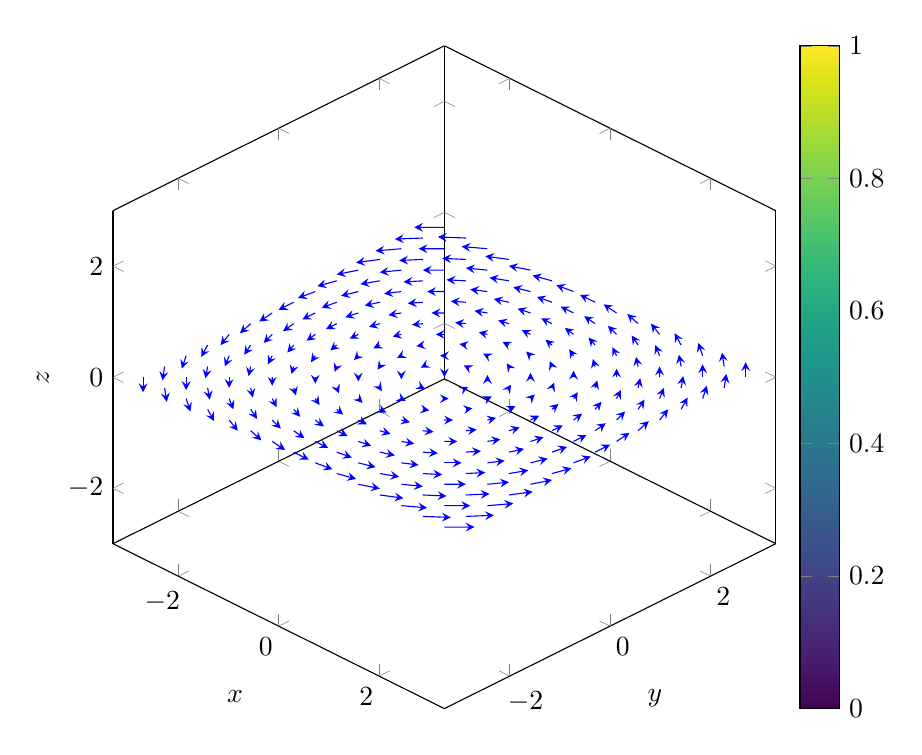
\begin{tikzpicture}
\centering
\begin{axis}[
    width=10cm,
    height=10cm,
    view={45}{35},
    domain=-3:3,
    y domain=-3:3,
    zmin=-3.0,
    zmax=3.0,
    xlabel={$x$},
    ylabel={$y$},
    zlabel={$z$},
    colorbar,
    colormap/viridis,
    ]
    % Definicja pola wektorowego
    \addplot3[blue,
    quiver={
     u={-y},
     v={x},
     w={0.5*z},
     scale arrows=0.1,
    },
    -stealth,samples=15]
    {0};
\end{axis}
\end{tikzpicture}

Podstawowe operacje na tym polu obejmują różniczkowanie i całkowanie wektorów. Kluczowe z nich to:
\begin{itemize}
    \item \textbf{Gradient:} jest operacją, która przypisuje każdemu punktowi przestrzeni wektor wskazujący kierunek i szybkość największego wzrostu danej funkcji skalarnej.
    \item \textbf{Dywergencja:} mierzy miarę źródła lub ujścia pola wektorowego w danym punkcie, tj. jak bardzo pole "rozchodzi się" z tego punktu.
    \item \textbf{Rotacja:} określa obrót pola wektorowego wokół danego punktu. 
    \item \textbf{Laplasjan:} jest operacją drugiego rzędu, która mierzy różnicę między wartością funkcji w danym punkcie a jej średnią wartością wokół tego punktu. 
\end{itemize}
W kontekście sieci neuronowych, najbardziej interesującą dla nas operacją jest gradient. Gradient funkcji skalarniej \(f(x_1, x_2, ..., x_n)\) w \(n\)-wymiarowej przestrzeni euklidesowej jest wektorem wszystkich jej pierwszych cząstkowych pochodnych. Oznacza to, że gradient wskazuje kierunek najszybszego wzrostu funkcji w danym punkcie i jest określony jako:
\begin{equation}
\nabla f = \left( \frac{\partial f}{\partial x_1}, \frac{\partial f}{\partial x_2}, ..., \frac{\partial f}{\partial x_n} \right)
\end{equation}


Rozważmy funkcję \(f(x, y) = x^2 + y^2\). Jest to prosta funkcja skalarna, której gradient w dowolnym punkcie \((x, y)\) wskazuje kierunek najszybszego wzrostu wartości funkcji.

\begin{figure}[h]
\centering
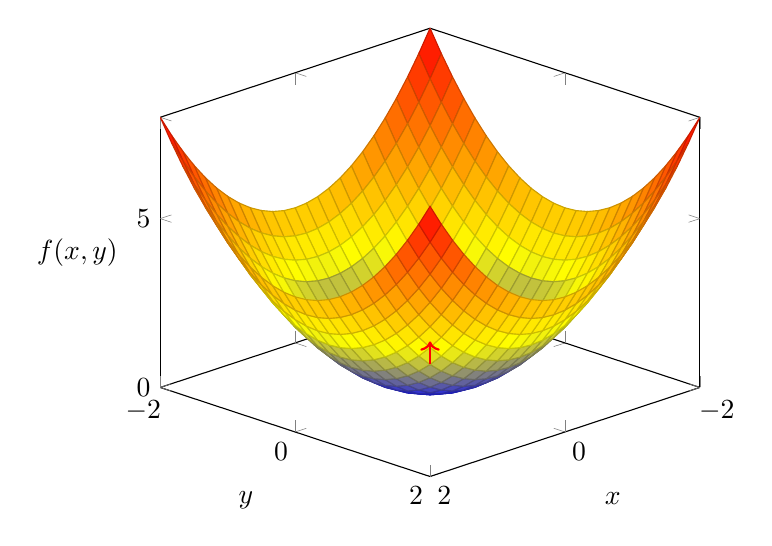
\begin{tikzpicture}
    \begin{axis}[
        xlabel=$x$, ylabel=$y$, zlabel={$f(x, y)$},
        zlabel style={rotate=-90},
        domain=-2:2,
        y domain=-2:2,
        zmin=0, zmax=8,
        view={135}{25},
        samples=25,
        ]
        % Rysowanie powierzchni
        \addplot3[surf] {x^2 + y^2};
        
        % Dodanie wektora gradientu w punkcie (1,1)
        \draw[->, thick, red] (axis cs:1,1,2) -- (axis cs:2,2,4);
    \end{axis}
\end{tikzpicture}
\caption{Wizualizacja gradientu}
\end{figure}
Gradient jest szczególnie wykorzystywany w uczeniu sieci neuronowych, bowiem szukamy jego minimum dla zadanych wag i biasów w stosunku do funkcji kosztu, w przypadku rysunku 1.2 jest to obszar zacieniowany na ciemnoniebiesko.
Kolejnymi szczególnie ważną operacją w sieciach neuronowych a konkretnie w uczeniu głębokim (ang. \textit{Deep Learning}) jest reguła łańcuchowa. Najpierw zdefiniujmy sobie funkcję żlożoną \(f \circ g\) dwóch funkcji \(f: Y \rightarrow Z\) i \(g: X \rightarrow Y\) jest definiowana jako:
\begin{equation}
    (f \circ g)(x) = f(g(x))
\end{equation}
dla każdego \(x \in X\).
Reguła łańcuchowa służy do obliczania pochodnej funkcji złożonej. Dla funkcji \(y = f(u)\) i \(u = g(x)\), pochodna funkcji złożonej \(y\) względem \(x\) jest dana przez:
\begin{equation}
    \frac{dy}{dx} = \frac{dy}{du} \cdot \frac{du}{dx}
\end{equation}

Dla złożenia \(n\) funkcji, pochodna funkcji złożonej \(y\) względem \(x\) obliczana jest jako:
\begin{equation}
    \frac{dy}{dx} = \frac{dy}{df_{n-1}} \cdot \frac{df_{n-1}}{df_{n-2}} \cdot \ldots \cdot \frac{df_2}{df_1} \cdot \frac{df_1}{dx}
\end{equation}
Znając już wyżej wymienione narzędzia możemy przedstawić schemat działania sieci neuronowych (rysunek poniżej). 
\begin{figure}[htbp]
\centering
\tikzset{%
  every neuron/.style={
    circle,
    draw,
    minimum size=1cm
  },
  neuron missing/.style={
    draw=none, 
    scale=4,
    text height=0.333cm,
    execute at begin node=\color{black}$\vdots$
  },
}
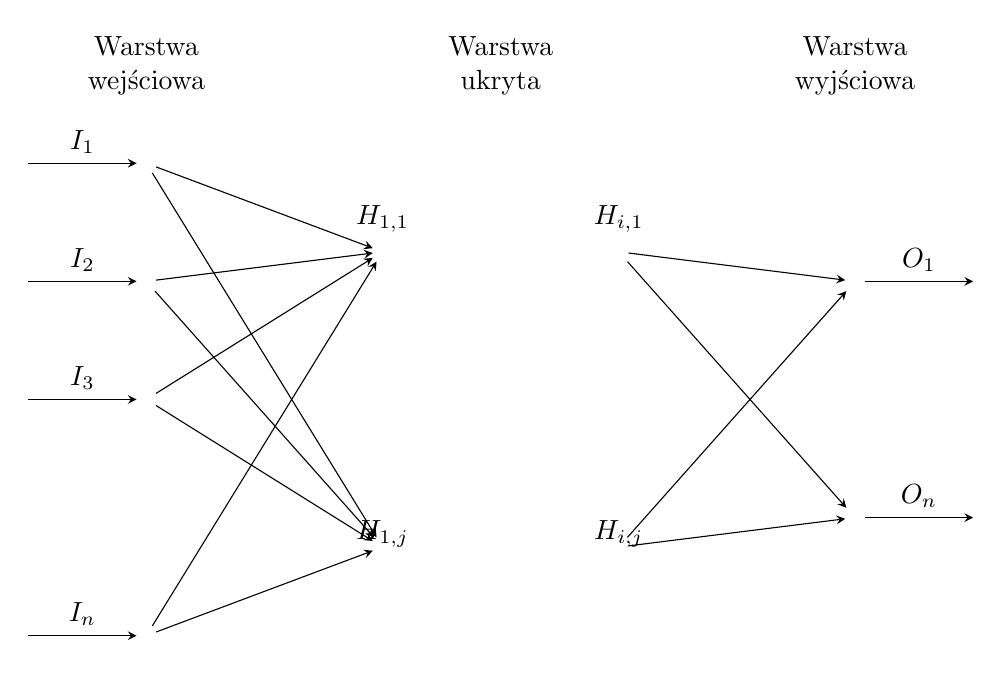
\begin{tikzpicture}[x=1.5cm, y=1.5cm, >=stealth]

% Wejście
\foreach \m/\l [count=\y] in {1,2,3,missing,4}
  \node [every neuron/.try, neuron \m/.try] (input-\m) at (0,2.5-\y) {};

% Pierwsza warstwa ukryta
\foreach \m [count=\y] in {1,missing,2}
  \node [every neuron/.try, neuron \m/.try ] (hidden1-\m) at (2,2-\y*1.25) {};

% Ostatnia warstwa ukryta
\foreach \m [count=\y] in {1,missing,2}
  \node [every neuron/.try, neuron \m/.try ] (hiddenN-\m) at (4,2-\y*1.25) {};

% Wyjście
\foreach \m [count=\y] in {1,missing,2}
  \node [every neuron/.try, neuron \m/.try ] (output-\m) at (6,1.5-\y) {};

% Połączenia
\foreach \i in {1,...,4}
  \foreach \j in {1,...,2}
    \draw [->] (input-\i) -- (hidden1-\j);

\foreach \i in {1,...,2}
  \foreach \j in {1,...,2}
    \draw [->] (hiddenN-\i) -- (output-\j);

% Oznaczenia
\foreach \l [count=\i] in {1,2,3,n}
  \draw [<-] (input-\i) -- ++(-1,0)
    node [above, midway] {$I_{\l}$};

% Indeksowanie neuronów w warstwach ukrytych
\node [above] at (hidden1-1.north) {$H_{1,1}$};
\node [above] at (hidden1-2.south) {$H_{1,j}$};
\node [above] at (hiddenN-1.north) {$H_{i,1}$};
\node [above] at (hiddenN-2.south) {$H_{i,j}$};

\foreach \l [count=\i] in {1,n}
  \draw [->] (output-\i) -- ++(1,0)
    node [above, midway] {$O_{\l}$};

% Etykiety warstw
\node [align=center, above] at (0,2) {Warstwa\\wejściowa};
\node [align=center, above] at (3,2) {Warstwa\\ukryta};
\node [align=center, above] at (6,2) {Warstwa\\wyjściowa};

\end{tikzpicture}
\caption{Schemat sieci neuronowej z \(n\) warstwami ukrytymi, gdzie $H_{i,j}$ }
\end{figure}

Poniżej znajduję się wytłumaczenie zmiennych
\begin{itemize}
    \item \(I_n\) - symbolizuje n-te wejście do sieci neuronowej. Wejścia te są punktem startowym przepływu informacji przez sieć i mogą reprezentować różne cechy danych wejściowych.
    \item \(H_{i,j}\) - oznacza $j$-ty neuron w $i$-tej warstwie ukrytej. Neurony te przetwarzają informacje otrzymane z warstwy wejściowej i z poprzednich warstw ukrytych, potencjalnie w bardzo złożony sposób, dzięki nieliniowym funkcjom aktywacji i zdolności do tworzenia złożonych abstrakcji.
    \item \(O_n\) - reprezentuje n-te wyjście sieci, czyli wynik przetwarzania danych wejściowych przez sieć. W zależności od zadania, wyjścia te mogą reprezentować klasy w problemach klasyfikacji lub wartości ciągłe w problemach regresji.
\end{itemize}

Poniżej znajduje się opis warstw
\begin{itemize}
    \item \textbf{Warstwa wejściowa} jest pierwszą warstwą sieci neuronowej, która odbiera dane wejściowe. Każdy neuron w tej warstwie odpowiada za jedną cechę danych wejściowych.
    \item \textbf{Warstwa ukryta} zawiera neurony, które nie są bezpośrednio widoczne z zewnątrz sieci. Neurony te przetwarzają informacje otrzymane z warstwy wejściowej, tworząc abstrakcyjne reprezentacje danych, które ułatwiają zadanie, np. klasyfikację czy regresję. Głębokość warstwy ukrytej, determinuje liczbę złożeń funkcji  (przyjmowanie jako argumentów wartości funkcji aktywacyjnej w sieci poprzedniej) 
    \item \textbf{Warstwa wyjściowa} dostarcza wynik działania sieci. Liczba neuronów w tej warstwie i rodzaj funkcji aktywacji zależą od specyficznego zadania, które ma realizować sieć.
\end{itemize}

W najbardziej ogólnej postaci sieć pokazaną na rysunku 1.3 możemy utożsamiać ze złożoną funkcją tensorową. Gdyż tensor jest uogólnieniem tablic wielowymiarowych, macierzy oraz skalarów. Tak więc na samym wstępie przekazywane są dane wejściowe do  warstwy ukrytej. Następnie do każdego neuronu w warstwie ukrytej obliczamy wynik funkcji aktywacyjnej, gdzie argumentem tej funkcji jest liniowa kombinacja wag i wejść zsumowane na końcu z biasem. 
\begin{equation}
    h = f\left(\sum_{i=1}^{n} w_i x_i + b\right)
\end{equation}

gdzie:
\begin{itemize}
    \item $h$ jest aktywacją neuronu,
    \item $f$ jest funkcją aktywacyjną,
    \item $w_i$ są wagami przypisanymi do każdego z $n$ sygnałów wejściowych $x_i$,
    \item $b$ jest wyrazem wolnym, zwanym również biasem.
\end{itemize}
Funkcje aktywacyjne decydują o decydują o aktywacji neuronów na podstawie przetworzonych sygnałów wejściowych. Poniżej znajduje się lista z najpopularniejszymi funkcjami aktywacyjnymi:

\begin{enumerate}[label=\textbf{\arabic*.}]
    \item \textbf{Funkcja sigmoidalna (Sigmoid)} - przekształca wejście na wartości w zakresie od 0 do 1, co jest przydatne, gdy oczekiwane wyjście to prawdopodobieństwo.
    \[ \sigma(x) = \frac{1}{1 + e^{-x}} \]
    
    \item \textbf{ReLU (Rectified Linear Unit)} - obecnie jedna z najczęściej używanych funkcji aktywacyjnych, ze względu na jej skuteczność w uczeniu głębokich sieci.
    \[ f(x) = \max(0, x) \]
    
    \item \textbf{Tangens hiperboliczny (Tanh)} - przekształca wejście na wartości w zakresie od -1 do 1, co czyni go bardziej użytecznym w niektórych zastosowaniach niż sigmoid.
    \[ \tanh(x) = \frac{e^{x} - e^{-x}}{e^{x} + e^{-x}} \]
    
    \item \textbf{Softmax} - często używana w ostatniej warstwie sieci neuronowej dla zadań klasyfikacyjnych, przypisując prawdopodobieństwa do różnych klas.
    \[ \text{Softmax}(z_i) = \frac{e^{z_i}}{\sum_{j} e^{z_j}} \]
    gdzie \(z_i\) to wartość wejściowa \(i\)-tego neuronu w warstwie, a sumowanie odbywa się po wszystkich neuronach w tej warstwie.
\end{enumerate}
Po obliczeniu wartosci funkcji z argumentu opisanego w równaniu 1.64, wartosci wynikowe przesyłane są dalej w ten sam proces. Oznacza to, że ponownie bierzemy tym razem wyniki tych poprzednich funkcji robimy z nich kombinacje linową nowych wag wraz z dodaniem biasa oraz przekazujemy to jako argument do zadanej funkcji aktywacyjnej dla każdego neuronu w danej warstwie ukrytej. Albo też, przekształcamy zadane nam wartości z tych funkcji jako ostatni argument (również w postaci opisanej równaniem 1.64) do ostatecznej funkcji aktywacyjnej interesującego nas wyniku. Na bazie predykcji teoretycznej porównujemy ją ze stanem rzeczywistym, pomocnym narzędziem tutaj jest funkcja kosztu. W zależności od charakterystyki zmiennej wynikowej, funkcja kosztu może przyjmować różną postać. Najważniejszym aspektem i właściwością jest to że, pozwala ocenić jak dobrze model dopasował się do danych. Dla zadań regresji, gdzie zmienna wynikowa jest ciągła, często stosuje się:

\begin{itemize}
    \item \textbf{Błąd średniokwadratowy (MSE - Mean Squared Error):}
    \[ MSE = \frac{1}{N} \sum_{i=1}^{N} (y_i - \hat{y}_i)^2 \]
    gdzie $y_i$ to wartości rzeczywiste, $\hat{y}_i$ to wartości przewidywane przez model, a $N$ to liczba obserwacji.
    
    \item \textbf{Błąd średni bezwzględny (MAE - Mean Absolute Error):}
    \[ MAE = \frac{1}{N} \sum_{i=1}^{N} |y_i - \hat{y}_i| \]
\end{itemize}
Dla zadań klasyfikacji, gdzie zmienna wynikowa jest kategoryczna, używa się innych funkcji kosztu, takich jak:

\begin{itemize}
    \item \textbf{Entropia krzyżowa (Cross-Entropy):} dla klasyfikacji binarnej:
    \[ BCE = -\frac{1}{N} \sum_{i=1}^{N} [y_i \log(\hat{y}_i) + (1 - y_i) \log(1 - \hat{y}_i)] \]
    i dla klasyfikacji wieloklasowej:
    \[ CE = -\frac{1}{N} \sum_{i=1}^{N} \sum_{c=1}^{C} y_{i,c} \log(\hat{y}_{i,c}) \]
    gdzie $y_{i,c}$ to wskaźnik, czy klasa $c$ jest prawidłową klasą dla obserwacji $i$, a $\hat{y}_{i,c}$ to przewidywane prawdopodobieństwo, że obserwacja $i$ należy do klasy $c$, $C$ to liczba klas.
\end{itemize}
Uzyskując wynik funkcji kosztu, po sprawdzeniu jak model dopasował się do interesującego nas zestawu danych, możemy przejść do najciekawszej części a mianowicie do algorytmu propagacji wstecznej. Algorytm ten służy do obliczenia wrażliwości zmiany każdej wagi $w_i_g$ oraz biasu $b_i_g$ w całej sieci neuronowej, na zmianę wartości funkcji kosztu. W istocie algorytm ten jest po prostu realizacją gradientu i reguły łańcuchowej, opisanej równaniem 1.63 oraz 1.60. Bowiem jak wspomniałem wcześniej sieć neuronowa jest tak naprawdę jedynie skomplikowaną funkcją matematyczną, służącą do aproksymacji nieliniowej. Poniżej przedstawiłem kroki w której wykonywana jest pojedyńcza realizacja tego algorytmu. 
\begin{enumerate}[label=\textbf{Krok \arabic*:}]
    \item \textbf{Przeprowadzenie propagacji w przód} przez sieć, aby obliczyć wyjście \(\hat{y}\) i funkcję kosztu \(\mathcal{L}(y, \hat{y})\).

    \item \textbf{Inicjacja propagacji wstecznej} przez obliczenie gradientu funkcji kosztu względem przewidywanego wyjścia sieci:
    \begin{equation*}
    \frac{\partial \mathcal{L}}{\partial \hat{y}}
    \end{equation*}

    \item \textbf{Obliczanie gradientów względem wag i biasów} w każdej warstwie, stosując regułę łańcuchową:
    Dla wagi \(w\) i biasu \(b\) w warstwie \(l\), gradienty są obliczane jako:
    \begin{align*}
    \frac{\partial \mathcal{L}}{\partial w} &= \frac{\partial \mathcal{L}}{\partial \hat{y}} \cdot \frac{\partial \hat{y}}{\partial a^{(l)}} \cdot \frac{\partial a^{(l)}}{\partial w} \\
    \frac{\partial \mathcal{L}}{\partial b} &= \frac{\partial \mathcal{L}}{\partial \hat{y}} \cdot \frac{\partial \hat{y}}{\partial a^{(l)}} \cdot \frac{\partial a^{(l)}}{\partial b}
    \end{align*}
    gdzie \(a^{(l)}\) to aktywacja w warstwie \(l\) przed zastosowaniem funkcji aktywacji, a \(\frac{\partial \hat{y}}{\partial a^{(l)}}\) to pochodna wyjścia sieci względem aktywacji tej warstwy.

    \item \textbf{Aktualizacja parametrów} sieci neuronowej:
    \begin{align*}
    w &:= w - \eta \frac{\partial \mathcal{L}}{\partial w} \\
    b &:= b - \eta \frac{\partial \mathcal{L}}{\partial b}
    \end{align*}
    gdzie \(\eta\) jest współczynnikiem uczenia w praktyce przyjmuje wartości między 0,0001 a 0,1.
\end{enumerate}
Cały proces jest powtarzany do momentu aż interesujące nas mierniki (np. F1, MSE itd.) będą miały zadowalającą dla nas precyzję. Zazwyczaj startujemy z losowymi wartościami parametrów, następnie aktualizujemy je w oparciu o wynik gradientu i wartość współczynnika uczenia, a następnie iterujemy ten proces określoną ilość razy. Wzór który podałem na aktualizacje parametrów jest prawdziwy, ale tylko dla gradientu prostego (dla całego zestawu danych). W praktyce ze względu na dosyć duży koszt obliczeniowy nie zawsze się stosuje akurat tą metodę. Poniżej znajduje się lista najpopularniejszych algorytmów gradientowych. 
\begin{enumerate}[label=\arabic*.]
    \item \textbf{Gradient Prosty (Batch Gradient Descent)}\\
    Aktualizacja parametrów:
    \[ \theta = \theta - \eta \cdot \nabla_\theta J(\theta) \]
    
    \item \textbf{Stochastyczny Gradient Prosty (SGD)}\\
    Aktualizacja parametrów dla każdej próbki:
    \[ \theta = \theta - \eta \cdot \nabla_\theta J(\theta; x^{(i)}, y^{(i)}) \]
    
    \item \textbf{Mini-Batch Gradient Descent}\\
    Aktualizacja parametrów dla każdego mini-batcha:
    \[ \theta = \theta - \eta \cdot \nabla_\theta J(\theta; X_{\text{mini-batch}}, Y_{\text{mini-batch}}) \]
    
    \item \textbf{Momentum}\\
    Aktualizacja parametrów z wykorzystaniem momentu:
    \begin{align*}
    v_t &= \gamma v_{t-1} + \eta \cdot \nabla_\theta J(\theta) \\
    \theta &= \theta - v_t
    \end{align*}
    
    \item \textbf{Nesterov Accelerated Gradient (NAG)}\\
    Aktualizacja parametrów z wyprzedzeniem:
    \begin{align*}
    v_t &= \gamma v_{t-1} + \eta \cdot \nabla_\theta J(\theta - \gamma v_{t-1}) \\
    \theta &= \theta - v_t
    \end{align*}
    
    \item \textbf{Adagrad}\\
    Aktualizacja parametrów z adaptacyjnym współczynnikiem uczenia:
    \[ \theta = \theta - \frac{\eta}{\sqrt{G_t + \epsilon}} \odot \nabla_\theta J(\theta) \]
    gdzie \(G_t\) to diagonalna macierz sumująca kwadraty gradientów do czasu \(t\), a \(\epsilon\) to mała stała zapobiegająca dzieleniu przez zero.
    
    \item \textbf{RMSprop}\\
    Aktualizacja parametrów z wygładzonymi kwadratami gradientów:
    \[ \theta = \theta - \frac{\eta}{\sqrt{E[g^2]_t + \epsilon}} \odot \nabla_\theta J(\theta) \]
    
    \item \textbf{Adam (Adaptive Moment Estimation)}\\
    Aktualizacja parametrów z momentami pierwszego i drugiego rzędu:
    \begin{align*}
    m_t &= \beta_1 m_{t-1} + (1 - \beta_1) \nabla_\theta J(\theta) \\
    v_t &= \beta_2 v_{t-1} + (1 - \beta_2) (\nabla_\theta J(\theta))^2 \\
    \hat{m}_t &= \frac{m_t}{1 - \beta_1^t}, \quad \hat{v}_t = \frac{v_t}{1 - \beta_2^t} \\
    \theta &= \theta - \frac{\eta}{\sqrt{\hat{v}_t} + \epsilon} \odot \hat{m}_t
    \end{align*}
\end{enumerate}
\label{subsec:podrozdzial-2-rzedu}
Zasadniczo co może się wydawać zaskoczeniem, jedną z pierwszych aplikacji sieci neuronowych było właśnie modelowanie rynków kapitałowych, już w latach 90 około 3 lata po odkryciu algorytmu propagacji wstecznej przez Yana LeCuna. A więc te metody wcale nie są innowatorskie na tej płaszczyźnie. Jest to kompletnie odmienne podejście, od tych które prezentowałem w poprzednich podrozdziałach, jednakże posiadające również silny potencjał prognostyczny. W kontekście modelowania zmienności cen aktywów, interesować nas będzie specyficzny rodzaj sieci neuronowych dedykowany dla szeregów czasowych. Konkretnie chodzi tu o Rekurencyjne Sieci Neuronowe (RNN), które poza pewnymi szczegółami w ogólności działają tak samo jak klasyczna sieć neuronowa. W tym sensie, że parametry również podlegają propagacji wstecznej, a argumenty są funkcją wyników poprzednich warstw. 
Teraz omówmy pojęcie rekurencyjnych sieci neuronowych
\section{Sterowanie stochastyczne}
\section{Arbitraż statystyczny}
\section{Teoria optymalizacji portfela}


`\chapter{Empiryczna budowa portfela}
\label{chap:empiryczna-budowa-portfela}

\section{Założenia i strategia inwestycyjna}
\label{sec:zalozenia-i-strategia-inwestycyjna}

\section{Podejście stochastyczne}
\label{sec:podejscie-stochastyczne}

\subsection{Dobór aktywów i wag portfela}
\label{subsec:dobor-aktywow-i-wag}

\subsection{Modelowanie równań momentów}
\label{subsec:modelowanie-rownan-momentow}

\subsection{Analiza predykcyjna}
\label{subsec:analiza-predykcyjna}

\section{Podejście algorytmiczne}
\label{sec:podejscie-algorytmiczne}

\subsection{Metody heurystyczne w doborze portfela}
\label{subsec:metody-heurystyczne-w-doborze-portfela}

\subsection{Algorytmy ewolucyjne w optymalizacji wag aktywów}
\label{subsec:algorytmy-ewolucyjne-w-optymalizacji}

\subsection{Zastosowanie sieci neuronowych do identyfikacji wzorców rynkowych}
\label{subsec:zastosowanie-sieci-neuronowych}

\subsection{Zastosowanie analizy skupień do segmentacji rynku}
\label{subsec:analiza-skupien-segmentacja}

\subsection{Algorytmy do oceny i zarządzania ryzykiem portfela}
\label{subsec:algorytmy-do-oceny-ryzyka}

\subsection{Automatyzacja procesów inwestycyjnych za pomocą algorytmów}
\label{subsec:automatyzacja-procesow-inwestycyjnych}

\subsection{Integracja zewnętrznych danych do analizy algorytmicznej}
\label{subsec:integracja-zewnetrznych-danych}

\subsection{Backtesting i walidacja strategii algorytmicznych}
\label{subsec:backtesting-i-walidacja-strategii}

\chapter{Wyniki oraz podsumowanie}
\label{chap:wyniki-oraz-podsumowanie}
\section{Wynik finansowy portfeli}
\section{Odporność systemów w czasie}
\section{Podsumowanie}


% Załączniki
% \appendix
% \include{dodatekA}
% \include{dodatekB}
% itd.

%##############################################################################
% Poniżej odnajdziesz spisy dołączane do dokumentu (w tym do spisu treści).
% Jesli nie chcesz wykorszystać któregoś z nich w pracy, zakomentuj go 
% (znakiem procenta % na początku linii)

% Bibliografia
\clearpage
\printbibliography[heading=bibintoc]
 
% Spis tabel
\clearpage
\cleardoublepage
\phantomsection
\addcontentsline{toc}{chapter}{\listtablename}
\listoftables

% Spis rysunków
\clearpage
\cleardoublepage
\phantomsection
\addcontentsline{toc}{chapter}{\listfigurename}
\listoffigures

% Spis kodów źródłowych
\cleardoublepage
\phantomsection
\addcontentsline{toc}{chapter}{\lstlistlistingname}
\lstlistoflistings

\end{document}